% Options for packages loaded elsewhere
\PassOptionsToPackage{unicode}{hyperref}
\PassOptionsToPackage{hyphens}{url}
%
\documentclass[
]{article}
\usepackage{amsmath,amssymb}
\usepackage{lmodern}
\usepackage{iftex}
\ifPDFTeX
  \usepackage[T1]{fontenc}
  \usepackage[utf8]{inputenc}
  \usepackage{textcomp} % provide euro and other symbols
\else % if luatex or xetex
  \usepackage{unicode-math}
  \defaultfontfeatures{Scale=MatchLowercase}
  \defaultfontfeatures[\rmfamily]{Ligatures=TeX,Scale=1}
\fi
% Use upquote if available, for straight quotes in verbatim environments
\IfFileExists{upquote.sty}{\usepackage{upquote}}{}
\IfFileExists{microtype.sty}{% use microtype if available
  \usepackage[]{microtype}
  \UseMicrotypeSet[protrusion]{basicmath} % disable protrusion for tt fonts
}{}
\makeatletter
\@ifundefined{KOMAClassName}{% if non-KOMA class
  \IfFileExists{parskip.sty}{%
    \usepackage{parskip}
  }{% else
    \setlength{\parindent}{0pt}
    \setlength{\parskip}{6pt plus 2pt minus 1pt}}
}{% if KOMA class
  \KOMAoptions{parskip=half}}
\makeatother
\usepackage{xcolor}
\IfFileExists{xurl.sty}{\usepackage{xurl}}{} % add URL line breaks if available
\IfFileExists{bookmark.sty}{\usepackage{bookmark}}{\usepackage{hyperref}}
\hypersetup{
  pdftitle={Defocus Corrected Large Area Cryo-EM (DeCo-LACE) for Label-Free Detection of Molecules across Entire Cell Sections},
  pdfauthor={Johannes ElferichNikolaus Grigorieff},
  pdflang={en-US},
  pdfkeywords={cryo-EM, visual protemics, ribosome},
  hidelinks,
  pdfcreator={LaTeX via pandoc}}
\urlstyle{same} % disable monospaced font for URLs
\usepackage{graphicx}
\makeatletter
\def\maxwidth{\ifdim\Gin@nat@width>\linewidth\linewidth\else\Gin@nat@width\fi}
\def\maxheight{\ifdim\Gin@nat@height>\textheight\textheight\else\Gin@nat@height\fi}
\makeatother
% Scale images if necessary, so that they will not overflow the page
% margins by default, and it is still possible to overwrite the defaults
% using explicit options in \includegraphics[width, height, ...]{}
\setkeys{Gin}{width=\maxwidth,height=\maxheight,keepaspectratio}
% Set default figure placement to htbp
\makeatletter
\def\fps@figure{htbp}
\makeatother
\setlength{\emergencystretch}{3em} % prevent overfull lines
\providecommand{\tightlist}{%
  \setlength{\itemsep}{0pt}\setlength{\parskip}{0pt}}
\setcounter{secnumdepth}{-\maxdimen} % remove section numbering
\newlength{\cslhangindent}
\setlength{\cslhangindent}{1.5em}
\newlength{\csllabelwidth}
\setlength{\csllabelwidth}{3em}
\newlength{\cslentryspacingunit} % times entry-spacing
\setlength{\cslentryspacingunit}{\parskip}
\newenvironment{CSLReferences}[2] % #1 hanging-ident, #2 entry spacing
 {% don't indent paragraphs
  \setlength{\parindent}{0pt}
  % turn on hanging indent if param 1 is 1
  \ifodd #1
  \let\oldpar\par
  \def\par{\hangindent=\cslhangindent\oldpar}
  \fi
  % set entry spacing
  \setlength{\parskip}{#2\cslentryspacingunit}
 }%
 {}
\usepackage{calc}
\newcommand{\CSLBlock}[1]{#1\hfill\break}
\newcommand{\CSLLeftMargin}[1]{\parbox[t]{\csllabelwidth}{#1}}
\newcommand{\CSLRightInline}[1]{\parbox[t]{\linewidth - \csllabelwidth}{#1}\break}
\newcommand{\CSLIndent}[1]{\hspace{\cslhangindent}#1}
\ifLuaTeX
\usepackage[bidi=basic]{babel}
\else
\usepackage[bidi=default]{babel}
\fi
\babelprovide[main,import]{american}
% get rid of language-specific shorthands (see #6817):
\let\LanguageShortHands\languageshorthands
\def\languageshorthands#1{}
\usepackage[margin=2cm]{geometry}
\usepackage{setspace}
\doublespacing
\usepackage{lineno}
\linenumbers
\usepackage{cleveref}


%% pandoc-fignos: environment for tagged figures
\newenvironment{fignos:tagged-figure}[1][]{
    \let\oldthefigure\thefigure
    \let\oldtheHfigure\theHfigure
    \renewcommand{\thefigure}{#1}
    \renewcommand{\theHfigure}{#1}
  }{
    \let\thefigure\oldthefigure
    \let\theHfigure\oldtheHfigure
    \addtocounter{figure}{-1}
  }
\ifLuaTeX
  \usepackage{selnolig}  % disable illegal ligatures
\fi

\title{Defocus Corrected Large Area Cryo-EM (DeCo-LACE) for Label-Free Detection of Molecules across Entire Cell Sections}
\author{}
\date{}

\begin{document}
\maketitle

This manuscript
(\href{https://jojoelfe.github.io/deco_lace_template_matching_manuscript/v/6a99bb6d7d1ae0bbee70874ab4b79ba22f7fe1ce/}{permalink})
was automatically generated
from \href{https://github.com/jojoelfe/deco_lace_template_matching_manuscript/tree/6a99bb6d7d1ae0bbee70874ab4b79ba22f7fe1ce}{jojoelfe/deco\_lace\_template\_matching\_manuscript@6a99bb6}
on May 20, 2022.

\hypertarget{authors}{%
\subsection{Authors}\label{authors}}

\begin{itemize}
\item
  \textbf{Johannes Elferich}
  
\includegraphics[width=0.16667in,height=0.16667in]{images/orcid.pdf}
  \href{https://orcid.org/0000-0002-9911-706X}{0000-0002-9911-706X}
  · 
\includegraphics[width=0.16667in,height=0.16667in]{images/github.pdf}
  \href{https://github.com/jojoelfe}{jojoelfe}
  RNA Therapeutic Institute, UMass Chan Medical School; HHMI
\item
  \textbf{Nikolaus Grigorieff}
  
\includegraphics[width=0.16667in,height=0.16667in]{images/orcid.pdf}
  \href{https://orcid.org/0000-0002-1506-909X}{0000-0002-1506-909X}
  · 
\includegraphics[width=0.16667in,height=0.16667in]{images/github.pdf}
  \href{https://github.com/nikogrigorieff}{nikogrigorieff}
  RNA Therapeutic Institute, UMass Chan Medical School; HHMI
\end{itemize}

\hypertarget{abstract}{%
\subsection{Abstract}\label{abstract}}

Localization of biomolecules inside a cell is an important goal of biological
imaging. Fluorescence microscopy can localize biomolecules inside whole cells
and tissues, but its ability to count biomolecules and accuracy of the spatial
coordinates is limited by the wavelength of visible light. Cryo-electron
microscopy (cryo-EM) provides highly accurate position and orientation
information of biomolecules but is often confined to small fields of view inside
a cell, limiting biological context. In this study we use a new data-acquisition
scheme called ``Defocus-Corrected Large-Area cryo-EM'' (DeCo-LACE) to collect
high-resolution cryo-EM data over entire sections (100 -- 200 nm thick lamellae)
of neutrophil-like mouse cells, representing 1-2\% of the total cellular
volume. We use 2D template matching (2DTM) to determine localization and orientation
of the large ribosomal subunit in these sections. These data provide ``maps'' of translational activity across
sections of mammalian cells. This new high-throughput cryo-EM
data collection approach together with 2DTM will advance visual
proteomics and complement other single-cell ``omics'' techniques, such as
flow-cytometry and single-cell sequencing.

\hypertarget{introduction}{%
\subsection{Introduction}\label{introduction}}

A major goal in understanding cellular processes is the knowledge of the
amounts, location, interactions, and conformations of biomolecules
inside the cell. This knowledge can be obtained by approaches broadly
divided into label- and label-free techniques. In label-dependent
techniques a probe is physically attached to a molecule of interest that
is able to be detected by its strong signal, such as a
fluorescent molecule. In label-free techniques, the physical properties
of molecules themselves are used for detection. An example for this is
proteomics using mass-spectrometry {[}\protect\hyperlink{ref-tSXIKPl7}{1}{]}. The advantage
of label-free techniques is that they can provide information over
thousands of molecules, while label-dependent techniques offer highly specific
information for a few molecules. Especially spatial information can
often only be achieved using label-dependent techniques, such as
fluorescence microscopy {[}\protect\hyperlink{ref-VBmW7Aot}{2}{]}.

Cryo-electron microscopy (cryo-EM) has the potential to directly visualize the
arrangement of atoms that compose biomolecules inside of cells, thereby
allowing label-free detection with high spatial accuracy. This has been
called ``visual proteomics'' {[}\protect\hyperlink{ref-tGQ6TSUo}{3}{]}. Since cryo-EM
requires thin samples (\textless500nm), imaging of biomolecules inside cells is
restricted to small organisms, thin regions of cells, or samples that
have been suitably thinned. Thinning can be achieved either by
mechanical sectioning {[}\protect\hyperlink{ref-g8QavfwP}{4}{]} or by
milling using a focused ion beam (FIB) {[}\protect\hyperlink{ref-16IhS1Nc4}{5}{]}. This complex workflow
leads to a low throughput of cryo-EM imaging of cells and is further
limited by the fact that at the required magnifications, typical fields
of view (FOV) are very small compared to mammalian cells, and the FOV
achieved by label-dependent techniques such as fluorescence light microscopy. The
predominant cryo-EM technique for the localization of biomolecules of
defined size and shape inside cells is cryo-electron tomography {[}\protect\hyperlink{ref-Rksh2dxu}{6}{]}. However, the requirement of a tilt series at
every imaged location and subsequent image alignment, severely limits
the throughput for molecular localization.

An alternative approach is to identify molecules by their structural
``fingerprint'' in single projection using ``2D template-matching'' (2DTM)
{[}\protect\hyperlink{ref-Ynb3IP6I}{7},\protect\hyperlink{ref-18KGpXYPE}{8},\protect\hyperlink{ref-10bXZuF3G}{9}{]}. In this
method, a 3D model of a biomolecule is used as a template to find 2D
projections that match the molecules visible in the electron
micrographs. This method requires a projection search on a fine angular
grid, and the projections are used to find local cross-correlation peaks
with the micrograph. Since the location of a biomolecule in the
z-direction causes predictable aberrations to the projection image, this
method can be used to calculate complete 3D coordinates and orientations
of a biomolecule in a cellular sample
{[}\protect\hyperlink{ref-18KGpXYPE}{8}{]}.

Here we apply 2DTM of the ribosome large subunit (LSU) to cryo-FIB milled
neutrophil-like murine cells {[}\protect\hyperlink{ref-1B9Vt9eYu}{10}{]}. We chose these
cells because genetic defects in the ribosome machinery often leads to
hematopoietic disease {[}\protect\hyperlink{ref-gRoY21jY}{11}{]} and direct quantification of
ribosome location, number and conformational states in hematopoietic cells could
lead to new insight into hematopoietic disease {[}\protect\hyperlink{ref-KAJ7221k}{12}{]}.
To increase the amount of collected data and to provide unbiased sampling of the
whole lamella, we devised a new data-acquisition scheme, ``Defocus-Corrected
Large Area Cryo-Electron microscopy'' (DeCo-LACE). 2DTM allows us to test whether
aberrations caused by large beam-image shifts and highly condensed beams
deteriorate the high-resolution signal. We find that these aberrations do not
impede LSU detection by 2DTM. The resulting data provide a description of
ribosome distribution in an entire lamella, which represent 1-2\% of the cellular
volume. We find a highly heterogeneous density of ribosomes within the cell.
Analysis of the throughput in this method suggests that for the foreseeable
future computation will be the bottleneck for visual proteomics.

\hypertarget{materials-and-methods}{%
\subsection{Materials and Methods}\label{materials-and-methods}}

\hypertarget{grid-preparation}{%
\subsubsection{Grid preparation}\label{grid-preparation}}

ER-HoxA9 cells were maintained in RPMI medium supplemented with 10\% FBS,
penicillin/streptomycin, SCF, and estrogen {[}\protect\hyperlink{ref-1B9Vt9eYu}{10}{]} at
37 °C and 5\% CO2. 120 h prior to grid preparation, cells were washed twice in PBS
and cultured in the same medium except without estrogen. Differentiation was
verified by staining with Hoechst-dye and inspection of nuclear morphology.
Cells were then counted and diluted to \(1\cdot10^6\) cells/ml. Grids (either 200
mesh copper grids, with a sillicone-oxide and 2 µm holes with a 2 µm spacing or
200 mesh gold grids with a thin gold film and 2 µm holes in 2 µm spacing) were
glow-discharged from both sides using a 15 mA for 45 s. 3.5 µl of cell suspension
was added to grids on the thin-film side and grids were blotted from the back
side using a GP2 cryoplunger (Leica) for 8 s and rapidly plunged into liquid
ethane at -185 °C.

\hypertarget{fib-milling}{%
\subsubsection{FIB-milling}\label{fib-milling}}

Grids were loaded into an Aquilos 2 FIB/SEM (Thermo Fisher) instrument with a
stage cooled to -190 °C. Grids were sputter-coated with platinum for 15 s at 45 mA
and then coated with a layer of platinum-precursor by opening the GIS-valve for
45 s. An overview of the grid was created by montaging SEM images and isolated
cells at the center of gridsquares were selected for FIB-milling. Lamellae were
generated automatically using the AutoTEM software (Thermo Fisher), with the
following parameters:

\begin{itemize}
\tightlist
\item
  Milling angle: 20°
\item
  Rough milling: 3.2 µm thickness, 0.5 nA current
\item
  Medium milling: 1.8 µm thickness, 0.3 nA current, 1.0° overtilt
\item
  Fine milling: 1.0 µm tchickness, 0.1 nA current, 0.5° overtilt
\item
  Finer milling: 700 nm thickness, 0.1 nA curent, 0.2° overtilt
\item
  Polish 1: 450 nm thickness, 50 pA current
\item
  Polish 2: 200 nm thickness, 30 pA current
\end{itemize}

This resulted in 6-10 µm wide lamella with 150-250 nm thickness as determined by
FIB-imaging of the lamella edges.

\hypertarget{data-collection}{%
\subsubsection{Data collection}\label{data-collection}}

Grids were loaded into a Titan Krios TEM (Thermo Fisher) operated at 300 keV and
equipped with a BioQuantum energy filter (Gatan) and K3 camera (Gatan). The
microscope was aligned using a cross-grating grid on the stage. Prior to each
session, we carefully performed the ``Image/Beam'' calibration in nanoprobe. We
set the magnification to a pixel size of 1.76 Å and condensed the beam to \textasciitilde{} 900 nm
diameter, resulting in the beam being completely visible on the camera. To
establish fringe-free conditions, the ``Fine eucentric'' procedure of SerialEM {[}\protect\hyperlink{ref-19ZFerhph}{13}{]} was
used to move a square of the cross-grating grid to the eucentric position of the
microscope. The effective defocus was then set to 2 µm, using the ``autofocus''
routine of SerialEM. The objective focus of the microscope was changed until no
fringes were visible. The stage was then moved in Z until images had an apparent
defocus of 2 µm. The difference in stage Z-position between the eucentric and
fringe-free conditions was used to move other areas into fringe-free condition.

Low magnification montages were used to find lamellae and lamellae that were
sufficiently thin and free of contamination were selected for automated data
collection. Overview images of each lamella were taken at 2250x magnification
(38 Å pixel size). The corners of the lamella in the overview image were manually
annotated in SerialEM and translated into beam image-shift values using SerialEM's
calibration. A hexagonal pattern of beam image-shift positions was calculated
that covered the area between the four corners in a serpentine way, with a
\(\sqrt{3}\cdot425\) nm horizontal spacing and \(3/4\cdot 850\) nm vertical spacing. Exposures were
taken at each position with a 30 e\textsuperscript{-}/Å\(^2\) total dose. After each exposure, the
defocus was estimated using the ctffind function of SerialEM and the focus for
the next exposure was corrected by the difference between the estimated focus
and the desired defocus of 800 nm. Furthermore, after each exposure the
deviation of the beam from the center of the camera was measured and corrected
using the ``CenterBeamFromImage'' command of SerialEM.

After data collection, a 20 s exposure at 2250x magnification of the lamella at
200 μm defocus was taken for visualization purposes. A Python script implementing
this procedure is available at {[}Link to repo{]}.

\hypertarget{deco-lace-data-processing}{%
\subsubsection{DeCo-LACE data processing}\label{deco-lace-data-processing}}

An overview of the data analysis pipeline is shown in Fig.
\ref{fig:deco_lace_workflow}.

\hypertarget{pre-processing}{%
\paragraph{Pre-processing}\label{pre-processing}}

Motion-correction, dose weighting and other preprocessing as detailed below was performed using \emph{cis}TEM {[}\protect\hyperlink{ref-MUY42yxp}{14}{]}. To avoid influence of the beam-edge on motion-correction, only a quarter of the
movie in the center of the camera was considered for calculation of the
estimated motion. After movie frames were aligned and summed, a mask for the
illuminated area was calculated by lowpass filtering the image with a 100 Å
resolution cutoff, thresholding the image at 10\% of the maximal value and then lowpass
filtering the mask again with a 100 Å resolution cutoff to smooth the mask edges. This mask was
then used to select dark areas in the image and fill the pixels with
Gaussian noise, with the same mean and standard deviation as the illuminated
area. A custom version of the unblur program {[}\protect\hyperlink{ref-1G4Y94qCy}{15}{]}
implementing this procedure is available at {[}link to decolace branch{]}. During motion correction images were resampled to a pixel size of 1.5 Å. The
contrast-transfer function (CTF) was estimated using ctffind
{[}\protect\hyperlink{ref-n43f3Sqs}{16}{]}, searching between 0.2 and 2 μm defocus.

\hypertarget{dtm}{%
\paragraph{2DTM}\label{dtm}}

The search template was generated from the atomic model of the mouse LSU
(PDB 6SWA, exluding the Epb1 subunit) using the cryo-EM simulator implemented in \emph{cis}TEM
{[}\protect\hyperlink{ref-q2PSamkS}{17}{]}. The
match\_template program {[}\protect\hyperlink{ref-10bXZuF3G}{9}{]} was used to search for this
template in the movie-aligned, exposure-filtered and masked images, using a 1.5°
angular step in out-of-plane angles and a 1.0° angular step in-plane. 11 defocus
planes in 20 nm steps centered around the ctffind-determined defocus were searched. Targets
were defined as detected when their matches with the template produced peaks
with a singal-to-noise ratio (SNR) above a threshold of 7.75, which was chosen
based on the one-false-positive-per-tile criterion {[}\protect\hyperlink{ref-Ynb3IP6I}{7}{]}.

\hypertarget{montage-assembly}{%
\paragraph{Montage assembly}\label{montage-assembly}}

The coordinates of each tile \(i\),
\(\mathbf{c}_{i}\) {[}2D Vector in pixels{]} were initialized using beam image-shift of the tile, \(\mathbf{b}_i\) {[}2D Vector in μm{]},
and the ISToCamera matrix \(\mathbf{IC}\), as calibrated by SerialEM:

\[\mathbf{c}_{i} = \mathbf{IC} \cdot \mathbf{b}_i\]

A list of tile pairs \(i,j\) that overlap were assembled by selecting images where
\(|\mathbf{c}_i-\mathbf{c}_j| < D_{Beam}\). In order to calculate the precise offset between tiles \(i\) and \(j\), \(\mathbf{r}_{i,j}\), we calculated the cross-correlation between the two tiles, masked to the overlapping illuminated area using the scikit-image
package {[}\protect\hyperlink{ref-stvWEJeu}{18}{]} was used to calculate refined offsets . The coordinates \(\mathbf{c}_{i}\) were then refined by a least-square minimization against \(\mathbf{r}_{i,j}\):

\[ \displaystyle{\min_{\mathbf{c}} \sum_{pairs}{(\mathbf{r}_{i,j} - (\mathbf{c}_i-\mathbf{c}_j))^2}}\]

using the scipy package {[}\protect\hyperlink{ref-8Miti2Gz}{19}{]}. The masked cross-correlation and the least-square minimization was repeated once more to arrive at the final tile alignment.

The x,y coordinates of target \(n\) detected by 2DTM in the tile \(i\),
\(\textbf{m}^\textrm{T}_{n,i}\), was transformed into the montage frame by adding
the coordinate of the tile.

\[ \textbf{m}^\textrm{M}_n = \textbf{m}^\textrm{T}_{n,i} + \textbf{c}_i\]

The z coordinate of each target was calculated as the sum of the defocus offset
for the target, the estimated defocus of the tile, and the nominal defocus of
the microscope when the tile was acquired.

Images were rendered using UCSF ChimeraX {[}\protect\hyperlink{ref-cYCuuZxG}{20}{]}. The Python scripts used for data processing are available
under {[}repolink{]}.

\hypertarget{results}{%
\subsection{Results}\label{results}}

\hypertarget{dtm-detects-large-ribosomal-subunits-in-cryo-fib-lamellae-of-mammalian-cells}{%
\subsubsection{2DTM detects large ribosomal subunits in cryo-FIB lamellae of mammalian cells}\label{dtm-detects-large-ribosomal-subunits-in-cryo-fib-lamellae-of-mammalian-cells}}

To test whether we could detect individual ribosomes in mammalian cells we
prepared cryo-lamellae of mouse neutrophil-like cells. An overview image
of a representative lamella clearly shows cellular features consistent with a
neutrophil-like phenotype, mainly a segmented nucleus and a plethora of
membrane-organelles, corresponding to the granules and secretory vesicles of
neutrophils (Fig. {[}\ref{fig:initmatching}{]}A). We then proceeded to acquire
micrographs on this lamella with a defocus of 0.5-1.0 μm, 30 e\textsuperscript{-}/Å\(^2\)/s
exposure and 1.76 Å pixel size. We manually selected multiple locations in the
lamella and acquired micrographs using standard low-dose techniques where
focusing is performed on a sacrificial area. The resulting micrographs showed
smooth bilayered membranes and no signs of crystalline ice (Fig.
{[}\ref{fig:initmatching}{]}C,D), indicating successful vitrification throughout the
lamella. Successful vitrification is facilitated by the small size (\textasciitilde8 μm diameter) of these cells.

We used an atomic model of the 60S mouse ribosomal subunit (6SWA) for 2DTM {[}\protect\hyperlink{ref-sbkam02a}{21}{]}. In a
subset of images, the distribution of cross-correlation scores significantly
exceeded the distribution expected from images devoid of detectable targets. In the
resulting scaled maximum-intensity projections (MIPs), clear peaks with SNR
values up to 10 were apparent (Fig. {[}\ref{fig:initmatching2}{]}A). Using a
threshold criterion to select significant targets (see Methods), we found that in
images of cytosolic compartments there were 10-500 ribosomes within one micrograph
(Fig. {[}\ref{fig:initmatching}{]}B-E). Notably, we found no targets in areas
corresponding to the nucleus (Fig. {[}\ref{fig:initmatching}{]}B) or mitochondria
(Fig. \protect\hyperlink{fig:initmatching}{1}D). In the cytoplasm, we found a highly variable
number of targets, only \textasciitilde{} 50 in some exposures (Fig. {[}\ref{fig:initmatching}{]}E) and
up to 500 in others (Fig. {[}\ref{fig:initmatching}{]}C). This is a ten-fold
difference in local ribosome concentration, highlighting the importance of
imaging larger areas of a lamella to gain a complete picture of target
distributions. We therefore set out to collect cryo-EM data for 2DTM from
mammalian cell lamellae in a high-throughput unbiased fashion.

\hypertarget{deco-lace-for-2d-imaging-of-whole-lamellae}{%
\subsubsection{DeCo-LACE for 2D imaging of whole lamellae}\label{deco-lace-for-2d-imaging-of-whole-lamellae}}

In order to obtain high-resolution data from complete lamellae, we used a new
approach for data collection. This approach uses three key strategies: (1) every
electron that exposes a fresh area of the sample is collected on the camera (2)
image shift is used to precisely and quickly raster the surface of a lamella and
(3) focusing is done without using a sacrificial area (Fig. {[}\ref{fig:approach}{]}A).

To ensure that every electron exposing a fresh area of the sample is captured by
the detector, we adjusted the electron beam size to be entirely contained by the
detector area. During canonical low-dose imaging, the microscope is configured so
that the focal plane is identical to the eucentric plane of the specimen stage.
This leaves the C2 aperture out of focus, resulting in ripples at the edge of
the beam (Fig. {[}\ref{fig:approach}{]}D). While these ripples are low-resolution
features that likely do not interfere with 2DTM {[}cite{]}, we also tested data
collection under conditions where the C2 aperture is in focus (``fringe-free'',
Fig. {[}\ref{fig:approach}{]}E).

We then centered a lamella on the optical axis of the microscope and used the
image shift controls of the microscope to systematically scan the whole surface
of the lamella in a hexagonal pattern (Fig. {[}\ref{fig:approach}{]}A,C). Instead of
focusing on a sacrificial area, we determined the defocus from every exposure
after it was taken. The defocus was then adjusted based on the difference
between desired and measured defocus (Fig. {[}\ref{fig:approach}{]}B). Since we used a
serpentine pattern for data collection, every exposure was close to the previous
exposure, making large changes in the defocus unlikely. Furthermore, we started
our acquisition pattern on the platinum deposition edge to make sure that the
initial exposure where the defocus was not yet adjusted did not contain any
biologically relevant information.

We used this strategy to collect data on eight lamellae, four using the
eucentric focus condition, hereafter referred to as Lamella\textsubscript{EUC}, and four using
the fringe-free condition, hereafter referred to as Lamella\textsubscript{FFF}(Fig.
{[}\ref{fig:assembly}{]} A+D, Fig.
{[}\ref{fig:lamella_images}{]}A). We were able to collect data with a highly
consistent defocus of 800 nm (Fig. {[}\ref{fig:approach}{]}F), both in the eucentric
focus and fringe-free focus condition. To ensure that data were collected
consistently, we mapped defocus values as a function of the applied image shift
(Fig. {[}\ref{fig:lamella_spatial_info}{]}A). This demonstrated that the defocus was
consistent across a lamella, except for rare outliers and in images containing
contamination. We also plotted the measured objective astigmatism of each
lamella and found that it varies with the applied image shift, becoming more
astigmatic mostly due to image shift in the x direction (Fig.
{[}\ref{fig:lamella_spatial_info}{]}B). While approaches exist to correct for this
during the data collection {[}\protect\hyperlink{ref-APSL9LmU}{22}{]}, we opted to not use these approaches in our
initial experiments. We reasoned that because 2DTM depends on high-resolution
information, this would be an excellent test of how much these aberration affect
imaging.

We assembled the tile micrographs into a montage using the image-shift values
and the SerialEM calibration followed by cross-correlation based refinement (see
Methods). In the resulting montages, the same cellular features visible in the
overview images are apparent (Fig. {[}\ref{fig:assembly}{]}B+E, Fig. {[}\ref{fig:lamella_images}{]}B), however
due to the high magnification and low defocus many more details, such as the
membrane bilayer separation, can be observed (Fig. {[}\ref{fig:assembly}{]}C+F). For montages collected using the
eucentric condition, there are clearly visible fringes at the edges between the
tiles (Fig. {[}\ref{fig:assembly}{]}C), which are absent in the fringe-free focus montages (Fig. {[}\ref{fig:assembly}{]}F). In our analysis
below, we show that these fringes do not impede target detection by 2DTM, making
them primarily an aesthetic issue. We also note that the tiling
pattern is visible in the montages (Fig. {[}\ref{fig:assembly}{]}B+E), which we believe is due to the non-linear
behavior of the K3 camera since we can observe these shading artifacts in micrographs of a condensed beam over vacuum (Fig. {[}\ref{fig:gain}{]}).

The montages show membrane vesicles and granules with highly variable sizes and
density. We found that a substantial number of granules, which are characterized by higher
density inside the the surrounding cytosol {[}\protect\hyperlink{ref-xE2EhAcH}{23}{]}, seemed to contain a membrane-enclosed inclusion with density similar to
the surrounding cytosol (Fig. {[}\ref{fig:lamella_images}{]}C) and could therefore be formed
by an autophagy-like pathway. These granules were
150-300 nm in diameter and the inclusions were 100-200 nm in diameter. Based on
these dimensions the granules are either azurophil or specific granules {[}\protect\hyperlink{ref-xE2EhAcH}{23}{]}. To our
knowledge, these inclusion have not been described in granulocytes and are
further described and discussed below.

\hypertarget{dtm-of-deco-lace-data-reveals-ribosome-distribution-in-cellular-cross-sections}{%
\subsubsection{2DTM of DeCo-LACE data reveals ribosome distribution in cellular cross-sections}\label{dtm-of-deco-lace-data-reveals-ribosome-distribution-in-cellular-cross-sections}}

In our initial attempts of using 2DTM on micrographs acquired with the DeCo-LACE
protocol, we did not observe any SNR peaks above threshold using the large
subunit of the mouse ribosome (Fig. {[}\ref{fig:crop_unblur}{]}A). We reasoned that
the edges of the beam might interfere with motion-correction of the movies as
they represent strong low-resolution features that do not move with the sample.
When we cropped the movie frames to exclude the beam edges, the estimated amount
of motion increased (Fig. {[}\ref{fig:crop_unblur}{]}B), consistent with successful
tracking of sample motion. Furthermore, in the motion-corrected average we could
identify significant SNR peaks (Fig. {[}\ref{fig:crop_unblur}{]}B), confirming to
high sensitivity of 2DTM to the presents of high-resolution signal preserved in
the images by the motion correction. To streamline data processing, we
implemented a function in unblur to consider only a defined central area of a
movie for estimation of sample motion, while still averaging the complete movie
frames (Fig. {[}\ref{fig:crop_unblur}{]}C). Using this approach, we motion-corrected
all tiles in the eight lamellae and found consistently total motion below 1 Å
per frame (Fig. {[}\ref{fig:lamella_motion_thickness}{]} A). In some lamellae we
found increased motion in the lamella center, which indicates areas of variable
mechanical stability within FIB-milled lamellae. In some micrographs we also
observed that the beam edges gave rise to artifacts in the MIP and numerous
false-positive detections at the edge of the illuminated area (Fig. {[}\ref{fig:crop_unblur}{]}D). A
similar phenomenon was observed on isolated ``hot'' pixels in unilluminated areas.
To overcome this issue we implemented a function in unblur to replace
dark areas in the micrograph with Gaussian noise (see Methods), with
mean and standard deviation matching the illuminated portion of the micrograph
(Fig. {[}\ref{fig:crop_unblur}{]}D+E). Together, these pre-processing steps enabled us to perform 2DTM on
all tiles of the eight lamellae.

We used the refined tile positions to calculate the positions of the detected
LSUs in the lamellae (Fig. {[}\ref{fig:matching_euc}{]}A, Fig. {[}\ref{fig:matching_fff}{]}A). Overlaying these positions of the lamellae montages reveal ribosome
distribution throughout the FIB-milled slices of individual cells. Organelles
like the nucleus and mitochondria only showed sporadic targets detected with low
SNRs, consistent with the estimated false-positive rate of one per tile. For
each detected target we also calculated the Z positions from the individual
estimated defocus and defocus offset for each tile. When viewed from the side,
the ribosome positions therefore show the slight tilts of the lamellae relative
to the microscope frame of reference (Fig. {[}\ref{fig:matching_euc}{]}B, Fig.
{[}\ref{fig:matching_fff}{]}B). Furthermore, the side views indicated that lamellae
were thinner at the leading edge. Indeed, when plotting the transmitted beam
intensities in individual tiles as a function of beam image-shift, we observed
substantially higher intensities at the leading edge (Fig. {[}\ref{fig:lamella_motion_thickness}{]}B), which in energy-filtered
TEM indicates a thinner sample {[}\protect\hyperlink{ref-17IP4Lhz1}{24}{]}. Even though we prepared the lamellae
with the ``overtilt'' approach {[}\protect\hyperlink{ref-hr3dyUeI}{25}{]}, this means that ribosome densities across
the lamellae can be skewed by a change in thickness, and better sample
preparation methods are needed to generate more even samples.

Close inspection of the ribosome positions in the lamellae revealed several
interesting features. Ribosomes could be seen associating with membranes, in
patterns reminiscent of the rough endoplasmic reticulum (Fig.
{[}\ref{fig:matching_euc}{]}C, Fig. {[}\ref{fig:matching_fff}{]}C) or the outer nuclear
membrane (Fig. {[}\ref{fig:matching_euc}{]}D). We also observed ribosomes forming
ring-like structures (Fig. {[}\ref{fig:matching_euc}{]}E), potentially indicating
circularized mRNAs {[}\protect\hyperlink{ref-cie13Q8F}{26}{]}. While ribosomes were for the most part excluded
from the numerous granules observed in the cytoplasm, in some cases we observed
clusters of ribosomes in the inclusions of double-membraned granules
described earlier (Fig. {[}\ref{fig:matching_euc}{]}F, Fig. {[}\ref{fig:matching_fff}{]}D,E). It is, in principle, possible that these targets are situated above or
below the imaged granules, since the granule positions in z cannot be determined
using 2D projections. However, in the case of Fig. {[}\ref{fig:matching_fff}{]}E, the
detected ribosomes span the whole lamella in the z direction (Fig. {[}\ref{fig:matching_fff}{]}F), while positions
above or below a granule would result in ribosomes situated exlusively at the
top or bottom of the lamella. This conclusive evidence of ribosomes in
inclusions is consistent with the earlier hypothesis that the inclusions are of
cytoplasmic origin.

\hypertarget{does-deco-lace-induce-aberrations-that-affect-2dtm}{%
\subsubsection{Does DeCo-LACE induce aberrations that affect 2DTM?}\label{does-deco-lace-induce-aberrations-that-affect-2dtm}}

Within the eight lamellae we found different number of detected targets (Fig.
{[}\ref{fig:matching_stat}{]}A). Lamella\textsubscript{EUC} 1 had the most detected targets, but also has
the largest surface area and contained cytoplasm from two cells. Lamella\textsubscript{FFF} 4
had the fewest detected targets, but this particular lamella was dominated by a
circular section of the nucleus, with only small pockets of cytoplasm (Fig.
{[}\ref{fig:lamella_images}{]}). In an attempt to normalize for these differences in
area containing cytoplasm, we compared the number of detected targets per tile in
tiles that contained more than one target, which should exclude tiles with
non-cytosolic content (Fig. {[}\ref{fig:matching_stat}{]}B). While this measure had
less variability, there were still differences. Lamella\textsubscript{EUC} 4 had not only the
fewest targets, but also the lowest density, which could be due to this lamella being the
thinnest, or due to it sectioning the cell in an area with a lower concentration of
ribosomes. Lamella\textsubscript{FFF} 3 had a substantially higher number of ribosomes per
tile. Since all of these lamellae were made from a cell-line under identical
conditions, this underscores the necessity to collect data from large numbers of
lamellae to overcome the inherent variability. When comparing the distribution of
scores between lamellae, we found them to be fairly comparable with median
SNRs ranging from 8.7 to 9.7 (Fig. {[}\ref{fig:matching_stat}{]}C). Lamella\textsubscript{EUC} 1 had slightly lower scores compared
to
the rest, potentially due to its large size and connected mechanical instability
during imaging. Overall, we did not observe differences in the number or SNR of
detected targets between eucentric or fringe-free illumination conditions that
were bigger than the observed inter-lamella variability.

Since the SNR values of 2DTM are highly sensitive to image quality, we reasoned
we could use them to verify that DeCo-LACE does not introduce a systematic loss
of image quality. We considered non-parallel illumination introduced by the
unusually condensed beam and uncharacterized aberrations near the beam
periphery. When plotting the SNR values of detected targets in all eight
lamellae as a function of their location in the tiles, we found uniformly high
SNR values throughout the illuminated areas for both eucentric and fringe-free
focus illumination, demonstrating that both illumination schemed are suitable
for DeCo-LACE (Fig. {[}\ref{fig:matching_stat}{]}D).

We also wondered whether large image shifts would lead aberration due to
astigmatism or beam tilt {[}\protect\hyperlink{ref-APSL9LmU}{22}{]}. We reasoned that if
that was the case the number of detected targets should be highest in the center of the
lamella where the applied beam image-shift is 0. Instead we observed that in
both eucentric and fring-free focus conditions more target where detected at the
``back'' edge of the lamella (Fig. {[}\ref{fig:matching_stat}{]}E{]}). This may be due to the center of the cell being predominantly
occupied by the nucleus, despite its segmentation in neutrophil-like cells. The
increase in matches at the ``back'' of the lamellae compared to the ``front'' can also
be explained by the thickness gradient of the lamellae (Fig. {[}\ref{fig:lamella_motion_thickness}{]}B,
Fig. {[}\ref{fig:matching_euc}{]}B, Fig. {[}\ref{fig:matching_fff}{]}B). In addition, aberrations would be expected to cause average 2DTM SNRs to be higher when beam-image shift
values are small. Instead, we found that SNRs where on average the highes at the
``front'' edge of the lamellae, presumably due to the thinner sample. We therefore
conclude that factors other that beam image-shift or beam
condensation aberrations are limiting 2DTM SNRS, predominantly the thickness of
the lamellae.

\hypertarget{computation-is-the-bottleneck-of-visual-proteomics}{%
\subsubsection{Computation is the bottleneck of visual proteomics}\label{computation-is-the-bottleneck-of-visual-proteomics}}

As described above, the variability of lamellae, both in terms of experimental
parameters including area, thickness and mechanical stability, and in terms of
biology, such as selection of cell type and location of the section within the
cell, requires collection of orders of magnitude more data than in this study to draw quantitative
and statistically relevant conclusions about the number and location of
molecules under different experimental conditions. The samples used were
prepared in two 24 h sessions on a FIB/SEM instrument, and imaging was performed
during another two 24h session on the TEM microscope. Inspections of the
timestamps of the raw data files revealed that the milling time per lamella was
\textasciitilde30 minutes and TEM imaging was accomplished in \textasciitilde10 seconds per tile or 90
minutes for a \textasciitilde{} 6x6 μm lamella. Processing of the data, however, took
substantially longer. Specifically, 2DTM of all tiles took approximately one
week per lamella on 32 A100 GPUs. Computation is therefore a bottleneck in our
current workflow, and further optimizations of the algorithm may be necessary
increase throughput. Alternatively, this bottleneck could be reduced by
increasing the number of processing units.

\hypertarget{discussion}{%
\subsection{Discussion}\label{discussion}}

In this study we developed an approach to image entire cellular cross-section using cryo-EM at high enough resolution to allow for 2DTM detection of the LSU. The two main advantages compared to previous approaches are a high throughput of imaging and the biological context for detected molecules. The requirement to increase throughput in cryo-EM data collection of cellular samples has been recognized in the recent literature. Most approaches describeb so far are tailored towards tomography. Peck et al. {[}\protect\hyperlink{ref-1GPPSX111}{27}{]} and Yang et al. {[}\protect\hyperlink{ref-ujizcpVn}{28}{]} developed approaches to increase the FOV of tomogram data-collection by using a montaging technique. Peck et al.~used a similar ``condensed-beam'' approach as described here. However, the montages are substantially smaller in scope, covering carbon film holes of 2 um diameter. Bouvette et al. {[}\protect\hyperlink{ref-1Gwx5ScUa}{29}{]} and Eisenstein et al. {[}\protect\hyperlink{ref-xvouNMBy}{30}{]} are using beam image-shift to collect tilt-series in multiple locations in parallel to increase throughput. However, none of these approaches provide the full coverage of a cellular cross-section that can be achieved using DeCo-Lace.

Since we observed substantial variation in ribosome density within and between lamellae, visual proteomics studies that use cryo-EM to establish changes in molecular organization within cells will require orders of magnitude more data than used in this study. One milestone would be to image enough data to represent one cellular volume, which for a small eukaryotic cells requires imaging approximately 100 lamella. While data collection throughput on the TEM is fundamentally limited by the exposure time, this amount of data could be collected within 12 hour by improving the data acquisition scheme to perform all necessary calculation in parallel with actual exposure of the camera. Sample preparation using a FIB/SEM is also currently a bottleneck, but preparation of large lamellae with multiple cellular cross-sections using methods like WAFFLE {[}\protect\hyperlink{ref-17H2LWiIu}{31}{]} might allow sufficient throughput. As stated in the results, at least for 2DTM computation will remain challenging and approximately 17,000 GPU hours would be required for a 100 lamellae dataset.

As described in {[}\protect\hyperlink{ref-Ynb3IP6I}{7}{]} the 2DTM SNR threshold for detecting a target is chosen to result in one false positive detection per image searched. We would therefore expect to find one false positive detection per tile. We reasoned that the large nuclear area imaged by DeCo-Lace could be used to test whether this assumption is true. In the 670 tiles containing exclusively nucleus (as manually annotated from the overview image) we detected 247 targets, making the false-positive rate more than twofold lower than expected. Since earlier work shows that 2DTM with the LSU can produce matches to nuclear ribosome biogenesis intermediates {[}\protect\hyperlink{ref-T1Qr0xyP}{32}{]}, this could even be an overestimate of the false-positive rate. This suggests that the detection threshold could be even lower, which is an area of ongoing research.

We found that even though we used beam image-shift extensively (up to 7 um), we did not see substantially reduced 2DTM SNR values in tiles acquired at high beam image-shift compared to tiles acquired with low or no beam image-shift. This is in contrast to reports in single-particle analysis (SPA) {[}\protect\hyperlink{ref-44fG6kcy}{33}{]} where the induced beam tilt substantially reduced the resolution if it was not corrected during processing. It is possible that 2DTM is less sensitive to beam-tilt aberrations, since the template is free of any aberration and only the image is distorted, while in SPA the beam tilt will affect both the images and the reconstructed template.

As mentioned in the results, we found a consistent shading artifact pattern in our montages, that we believe is the result of non-linear behavior of the K3 camera. Indeed, when we average images with a condensed beam taken over vacuum we found in both focus conditions a consistent background pattern with a brighter region on the periphery of the illuminated area (Fig {[}\ref{fig:gain}{]}). This might be caused by dynamic adjustment of the internal camera counting threshold which expects columns of the sensor to be evenly illuminated as is the case for SPA applications. Since the signal of this pattern has mainly low-resolution components it is unlikely to affect 2DTM. However, it highlights that the non-linear behavior of the camera has to be taken into account when imaging samples with strongly varying density and unusual illumination schemes.

Unexpectedly, we observed granules containing a vesicle of putative cytosolic origin. We speculate that upon degranulation, the process in which granules fuse with the plasma membrane, these vesicles would be released into the extracelullar space. The main types of extracellular vesicles of this size are exosomes, up to 100 nm large vesicles derived from fusion of multivesicular bodies with the plasma membrane, and microvesicles, which are derived from direct budding of the plasma membrane {[}\protect\hyperlink{ref-kncnYGLD}{34}{]}. We suggest that granulocytes could release a third type of extracellular vesicle, granule-derived vesicles (GDV), into the extracellular space. 2DTM showed that a subset of GDVs can contain ribosomes (Fig. {[}\ref{fig:matching_euc}{]}F, Fig. {[}\ref{fig:matching_fff}{]}D,E). This could indicate that these vesicles are transporting translation-capable mRNAs, as has been described for exosomes {[}\protect\hyperlink{ref-agVdpX76}{35}{]}. Further studies will be necessary to confirm the existence of GDVs in granulocytes isolated from mammals and to understand their functional significance.

\begin{figure}
\hypertarget{fig:deco_lace_workflow}{%
\centering
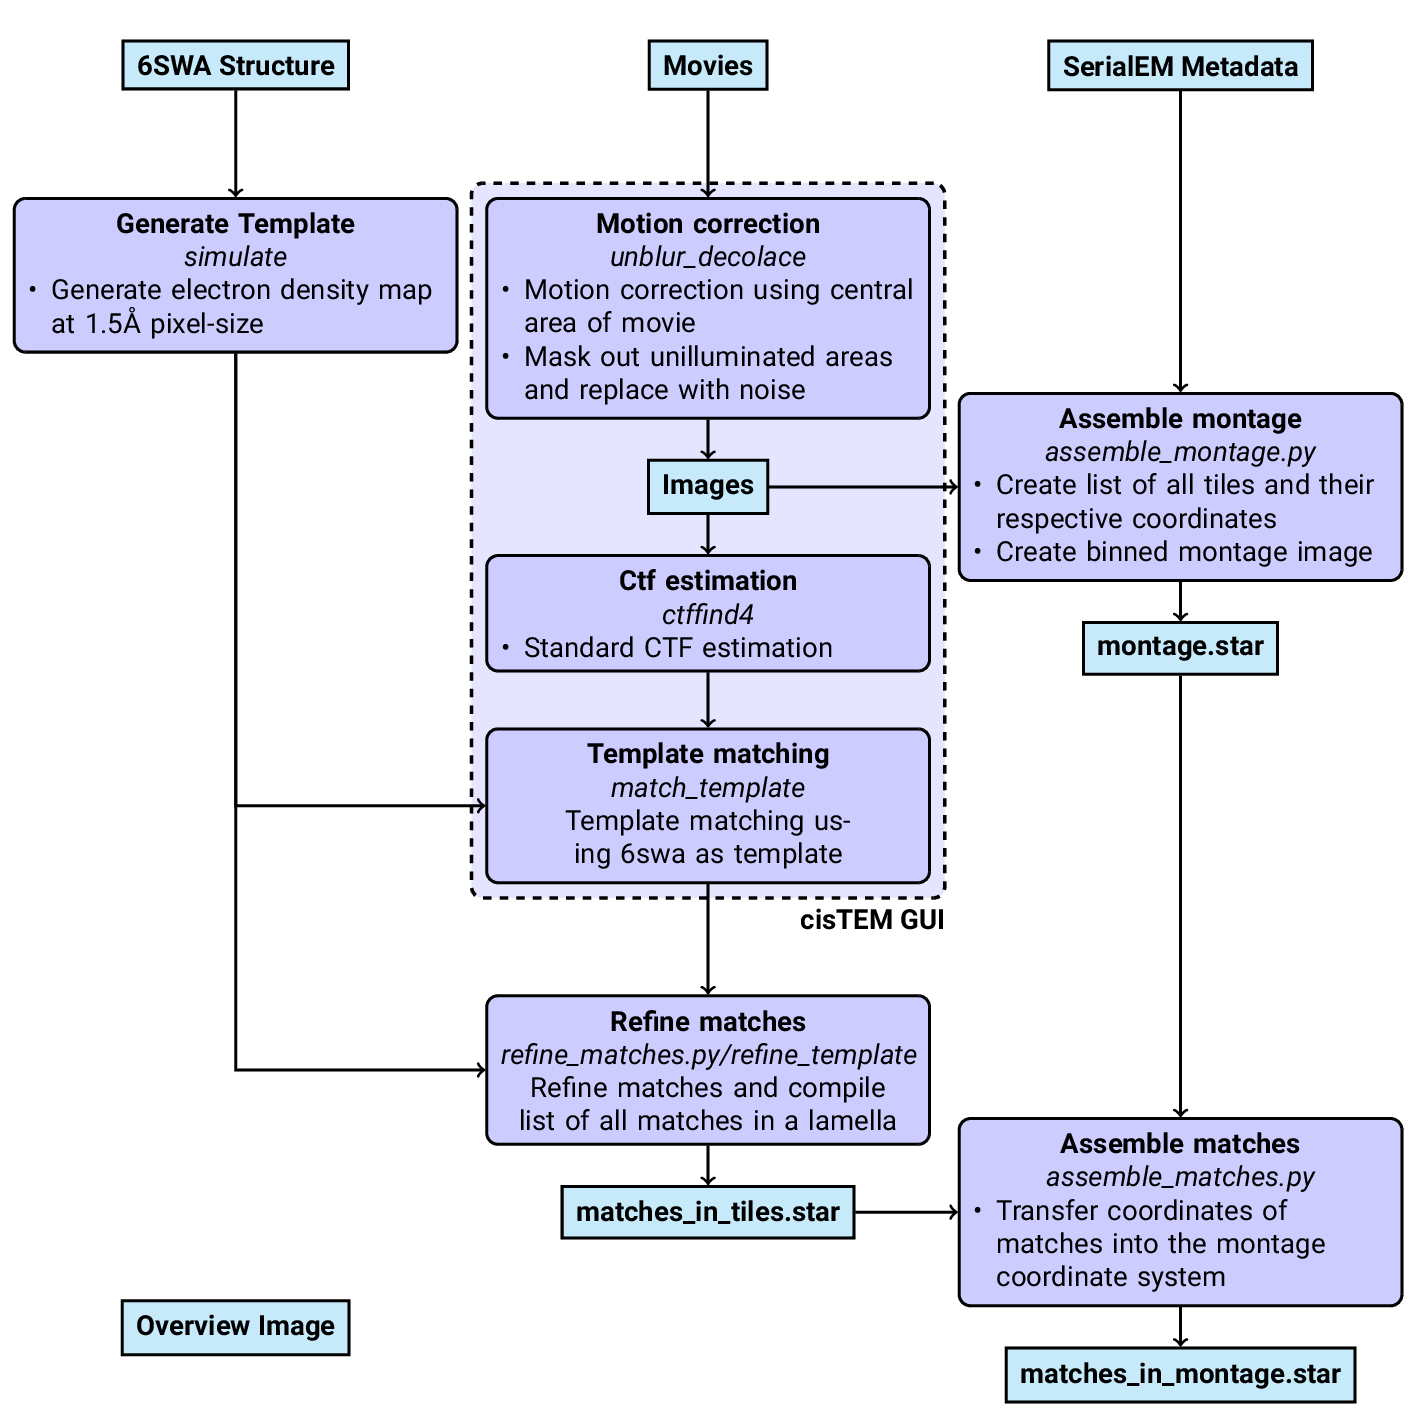
\includegraphics{figures/deco_lace_workflow.png}
\caption{Workflow of DeCo-Lace processing}\label{fig:deco_lace_workflow}
}
\end{figure}

\hypertarget{figures}{%
\subsection{Figures}\label{figures}}

\begin{figure}
\hypertarget{fig:initmatching}{%
\centering
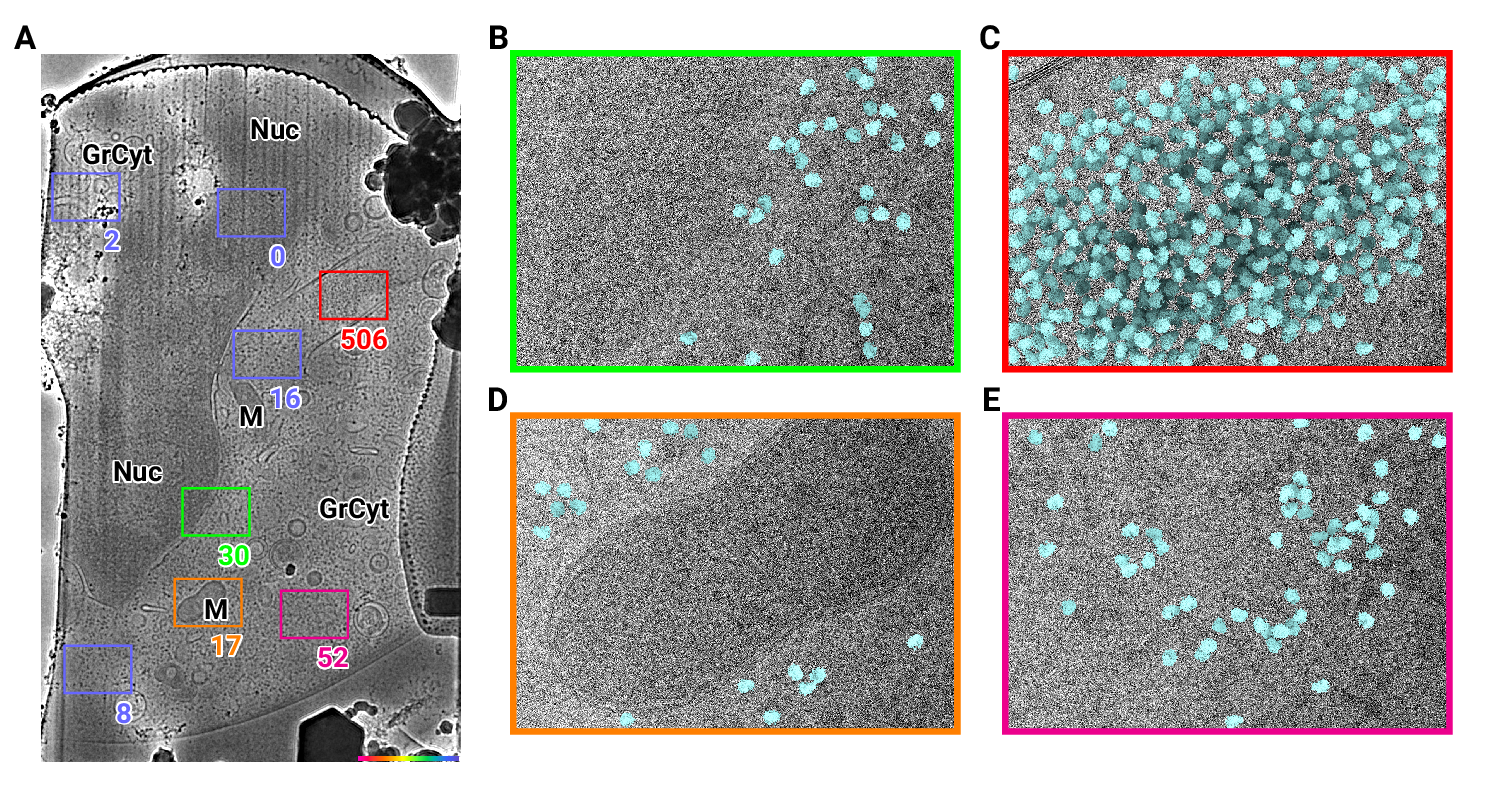
\includegraphics{figures/initmatching.png}
\caption{2D template matching of the large subunit of the ribosome in fib-milled neutrophil-like cells
(A) Overview image of the lamella. Major cellular regions are labeled, as Nucleus (Nuc), Mitochondria (M), and granular cytoplasm (GrCyt). FOVs where high-magnification images for template matching where acquired are indicated as boxes with the number of detected targets indicated on the bottom right. FOVs displayed in Panels B-E are color-coded. Scalebar corresponds to 1 μm.
(B-E) FOVs with projection of detected LSUs shown in cyan. (B) Perinuclear region, the only detected targets are in the cytoplasmic half. (C) Cytoplasmic region with high density of ribosomes (D) Mitochondrium, as expected there are only detected LSUs in the cytoplasmic region (E) Cytoplasm, with low density of ribosomes.}\label{fig:initmatching}
}
\end{figure}

\begin{fignos:tagged-figure}[2 - figure supplement 1]

\begin{figure}
\hypertarget{fig:initmatching2}{%
\centering
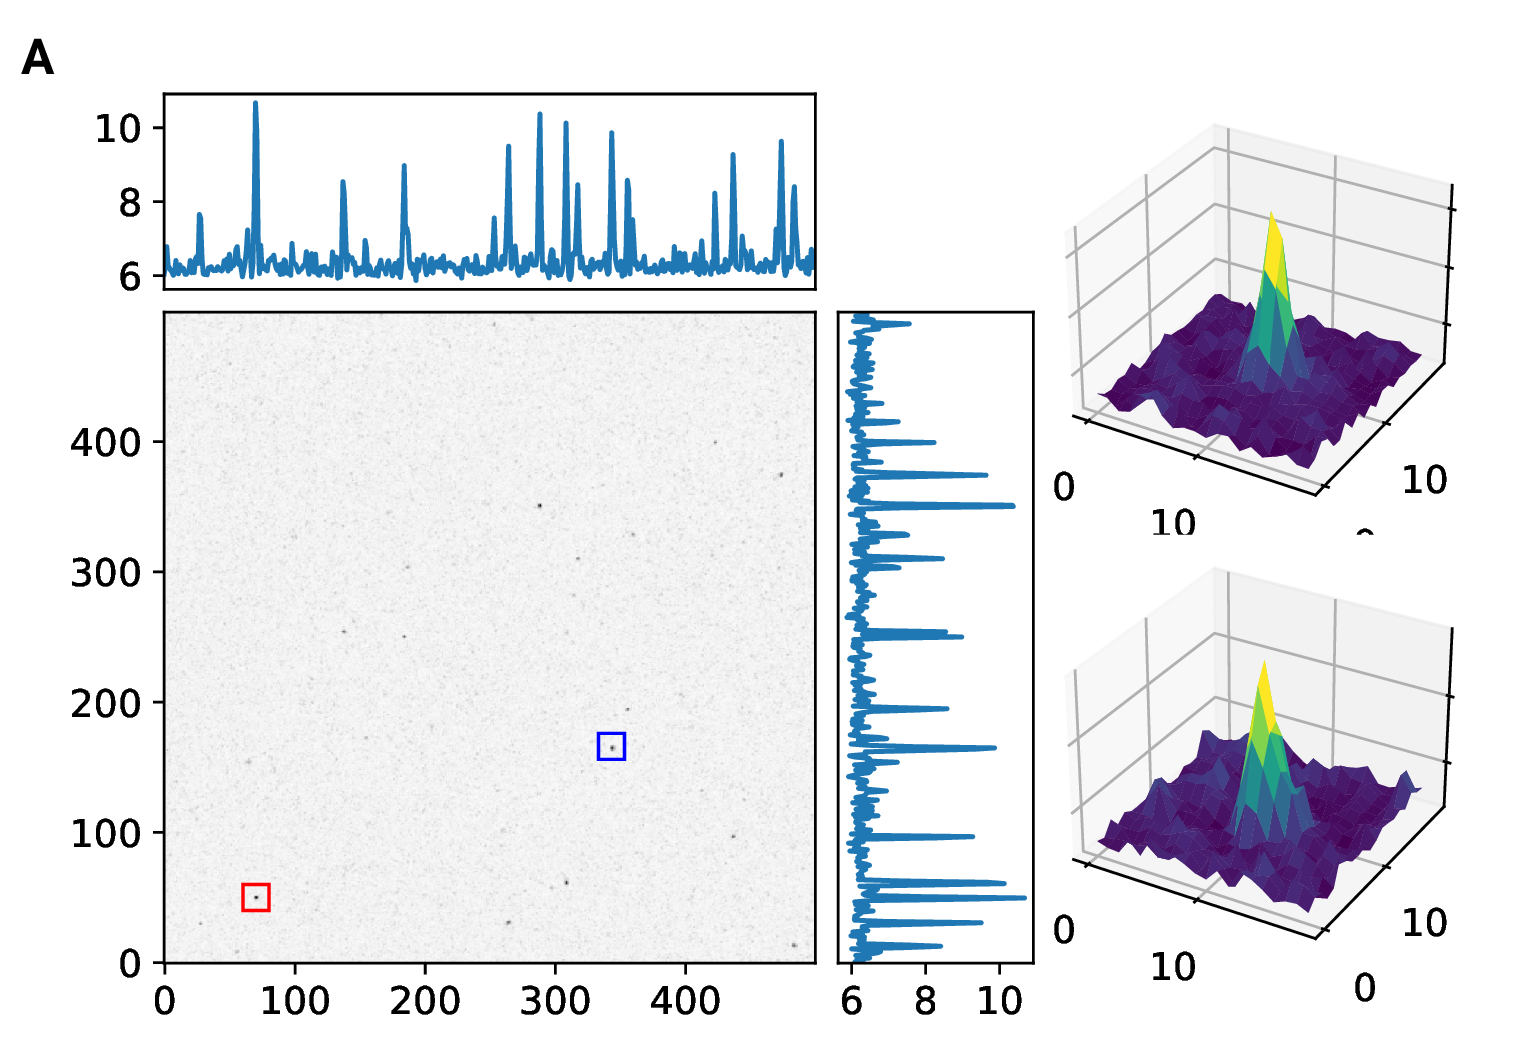
\includegraphics{figures/initmatching2.png}
\caption{2D template matching of the large subunit of the ribosome in fib-milled
neutrophil-like cells (A) Maximum intensity projection (MIP) cross-correlation map of
micrograph shown in Figure
\ref{fig:initmatching} (B+C) 3D plot of MIP regions indicated by color boxes in Panel A}\label{fig:initmatching2}
}
\end{figure}

\end{fignos:tagged-figure}

\begin{figure}
\hypertarget{fig:approach}{%
\centering
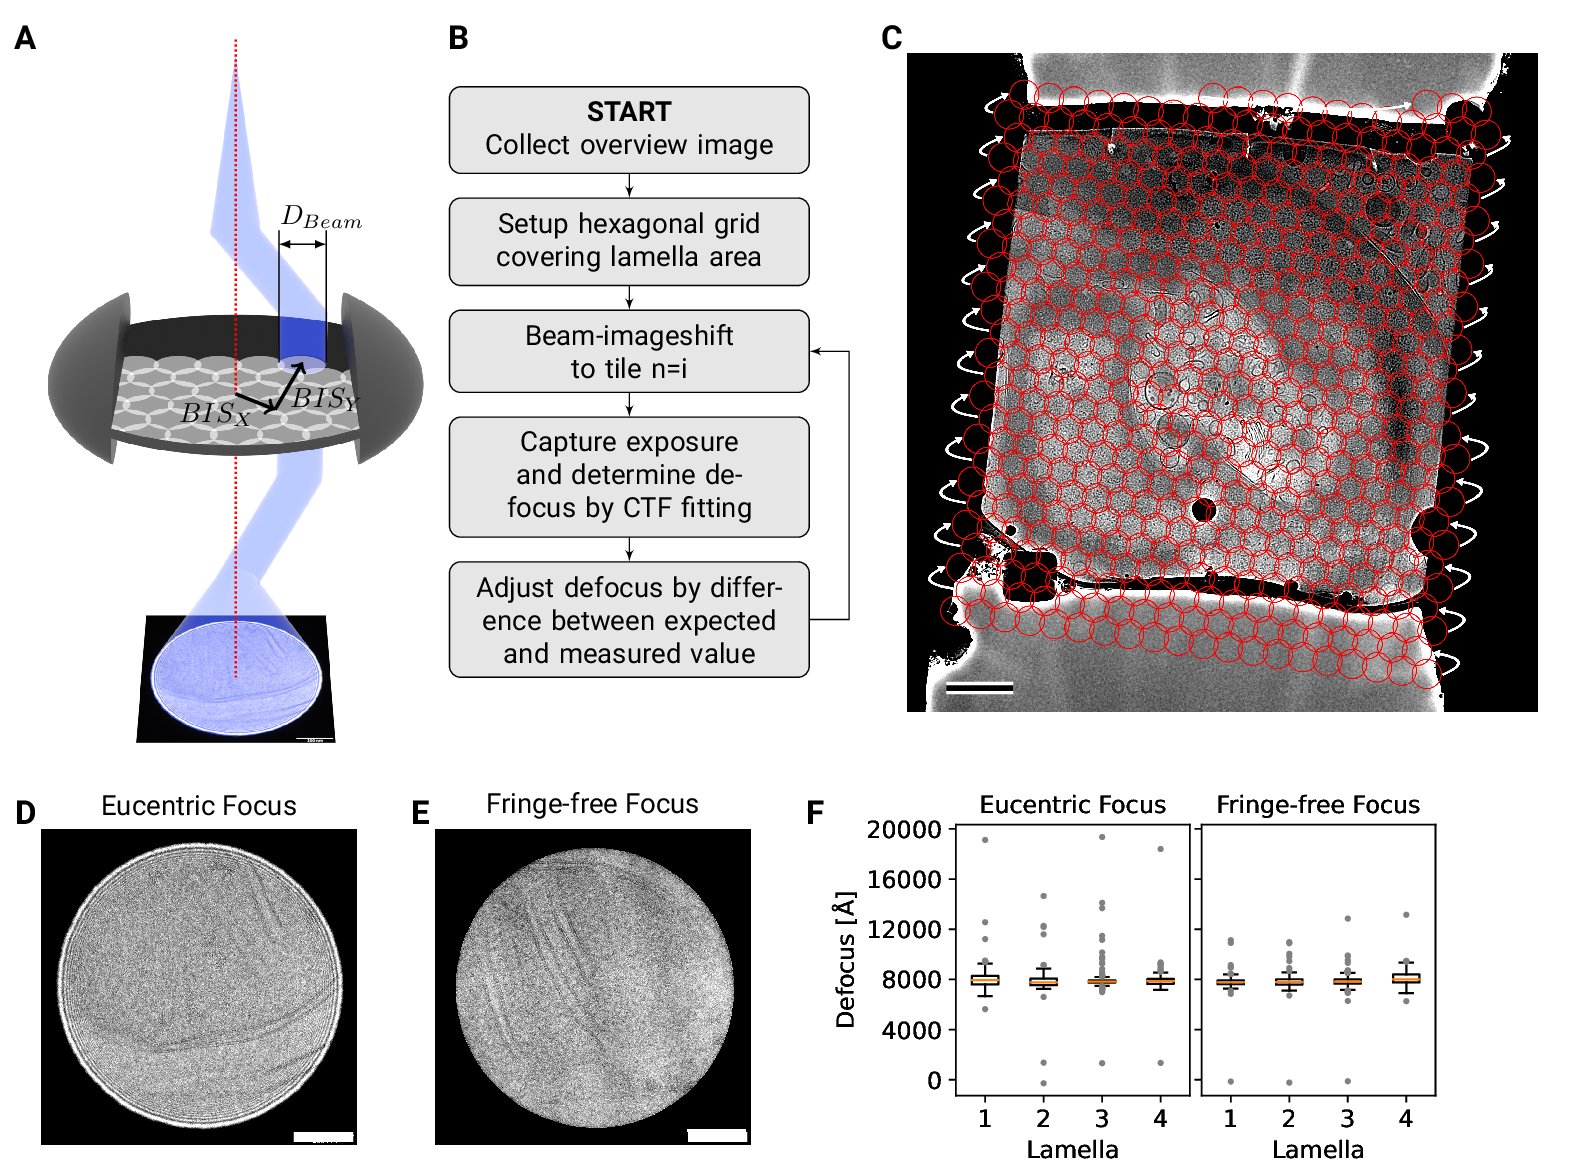
\includegraphics{figures/approach.png}
\caption{DeCo-LACE approach (A) Graphic demonstrating the data-collection strategy for
DeCo-LACE. The electron beam is condensed to a diameter \(D_{Beam}\) that allows captured of
the whole illuminated area on the camera. Beam-image shift along X and Y
(\(BIS_X\),\$\(BIS_Y\)) is used to scan the whole lamella
(B) Diagram of the collection algorithm
(C) Example overview image of a lamella with the designated acquisition
positions and the used beam diameter indicated with red circles. Scalebar corresponds to 1 μm.
(D+E) Representative micrographs takne with a condensed beam at eucentric focus
(D) or fringe-free focus (E). Scalebar corresponds to 100 nm.
(F) Boxplot of defocus measured by ctffind of micrographs taken by the DeCo-Lace
approach on four lamellae images at eucentric focus and four lamellae imaged with
fringe-free focus.}\label{fig:approach}
}
\end{figure}

\begin{fignos:tagged-figure}[3 - figure supplement 1]

\begin{figure}
\hypertarget{fig:lamella_spatial_info}{%
\centering
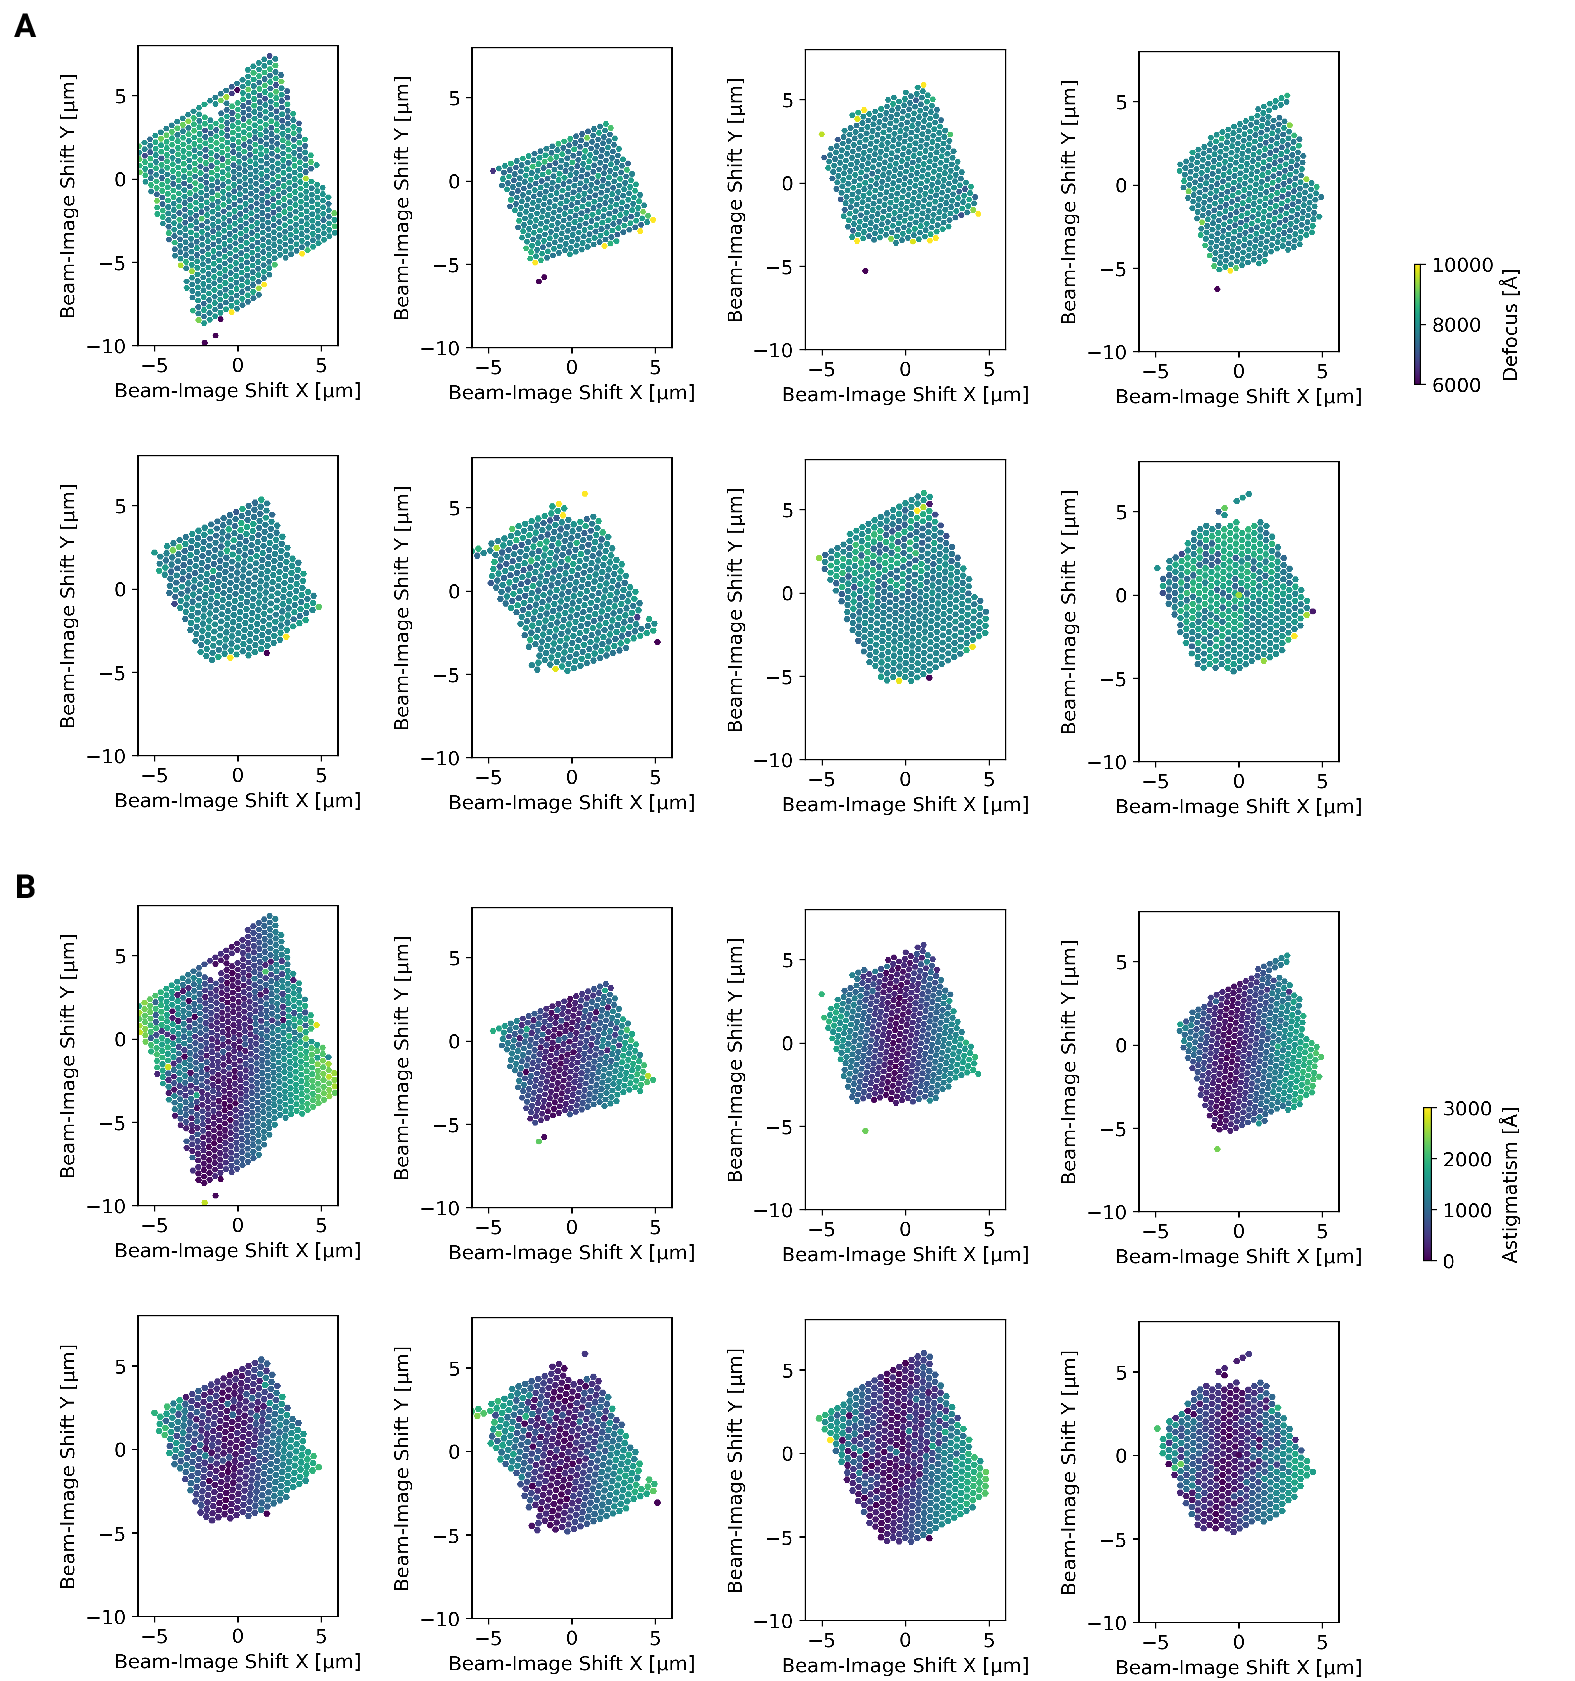
\includegraphics{figures/lamella_spatial_info.png}
\caption{Defocus estimation of individual tiles of DeCo-Lace montages
(A) Defocus values of individual micrographs taken using the DeCo-Lace approach
plotted as a function of the beam image-shift values.
(B) Defocus astigmatism of individual micrographs taken using the DeCo-Lace approach
plotted as a function of the beam image-shift values.}\label{fig:lamella_spatial_info}
}
\end{figure}

\end{fignos:tagged-figure}

\begin{figure}
\hypertarget{fig:assembly}{%
\centering
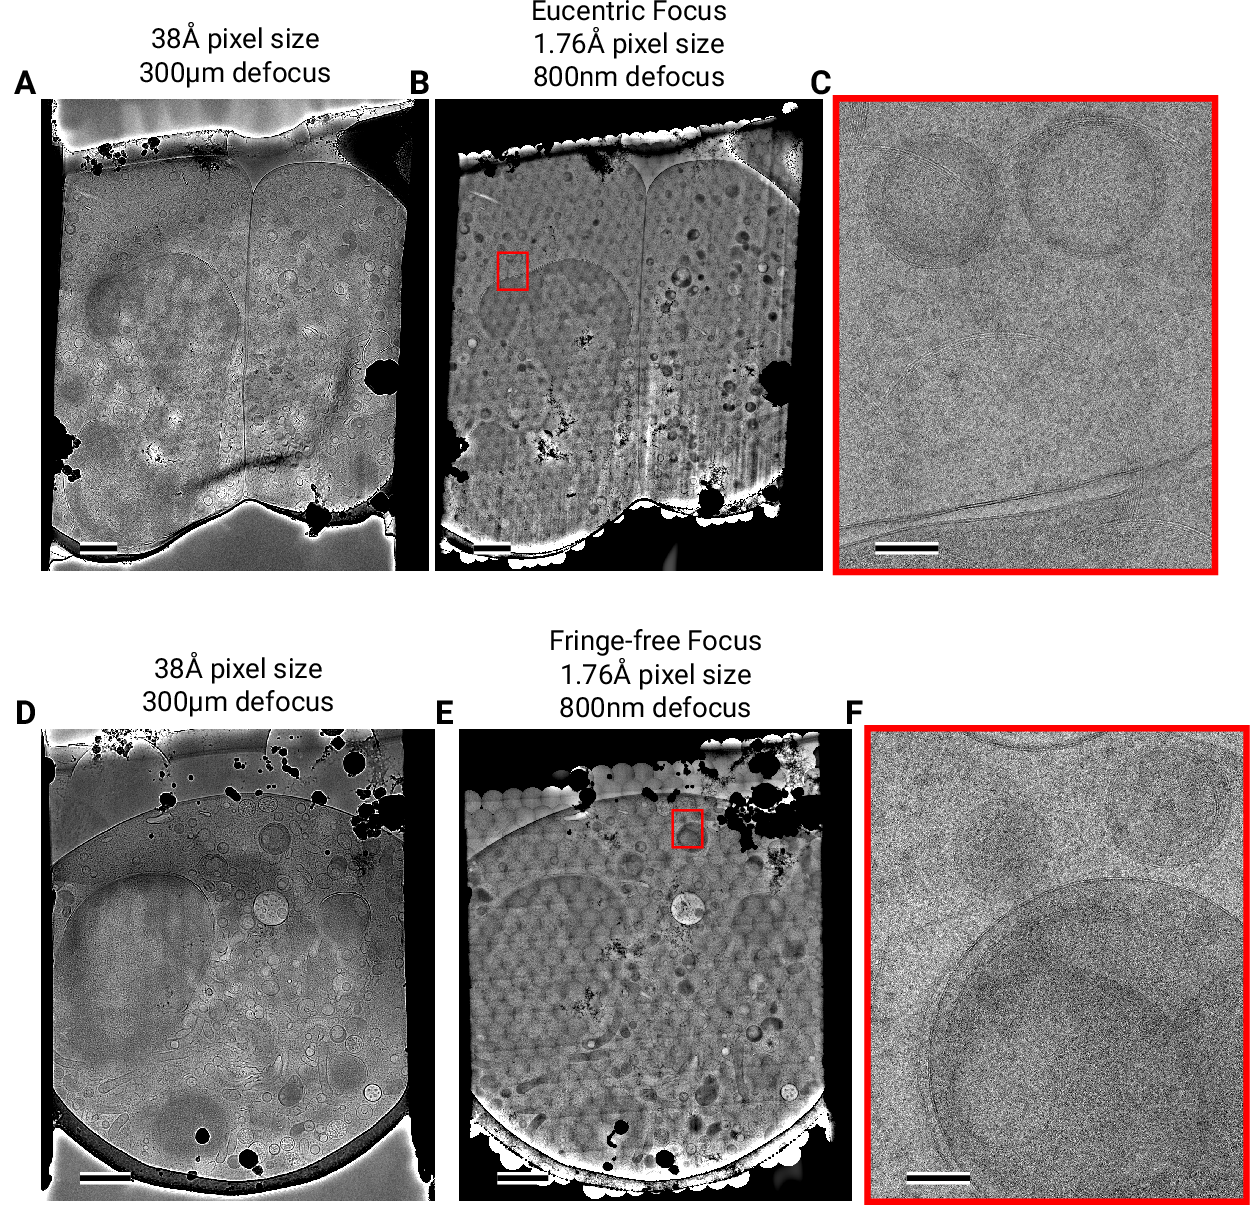
\includegraphics{figures/assembly.png}
\caption{Assembling DeCo-LACE exposures into montages (A) Overview
image of Lamella\textsubscript{EUC} 1 taken at low magnification. Scalebar corresponds to 1 μm. (B) Overview of Lamella\textsubscript{EUC} 1 created by
montaging high magnification images taken with the DeCo-Lace approach. Scalebar corresponds to 1 μm. (C) Zoom-in into red box in panel B. Slight beam-fringe artifacts are visible. Scalebar corresponds to 100 nm.
(D) Overview
image of Lamella\textsubscript{FFF} 4 taken at low magnification. Scalebar corresponds to 1 μm. (E) Overview of Lamella\textsubscript{FFF} 4 created by
montaging high magnification images taken with the DeCo-Lace approach. Scalebar corresponds to 1 μm. (F) Zoom-in into red box in panel E. No beam-fringe artifacts are visible. Scalebar corresponds to 100 nm.}\label{fig:assembly}
}
\end{figure}

\begin{fignos:tagged-figure}[4 - figure supplement 1]

\begin{figure}
\hypertarget{fig:crop_unblur}{%
\centering
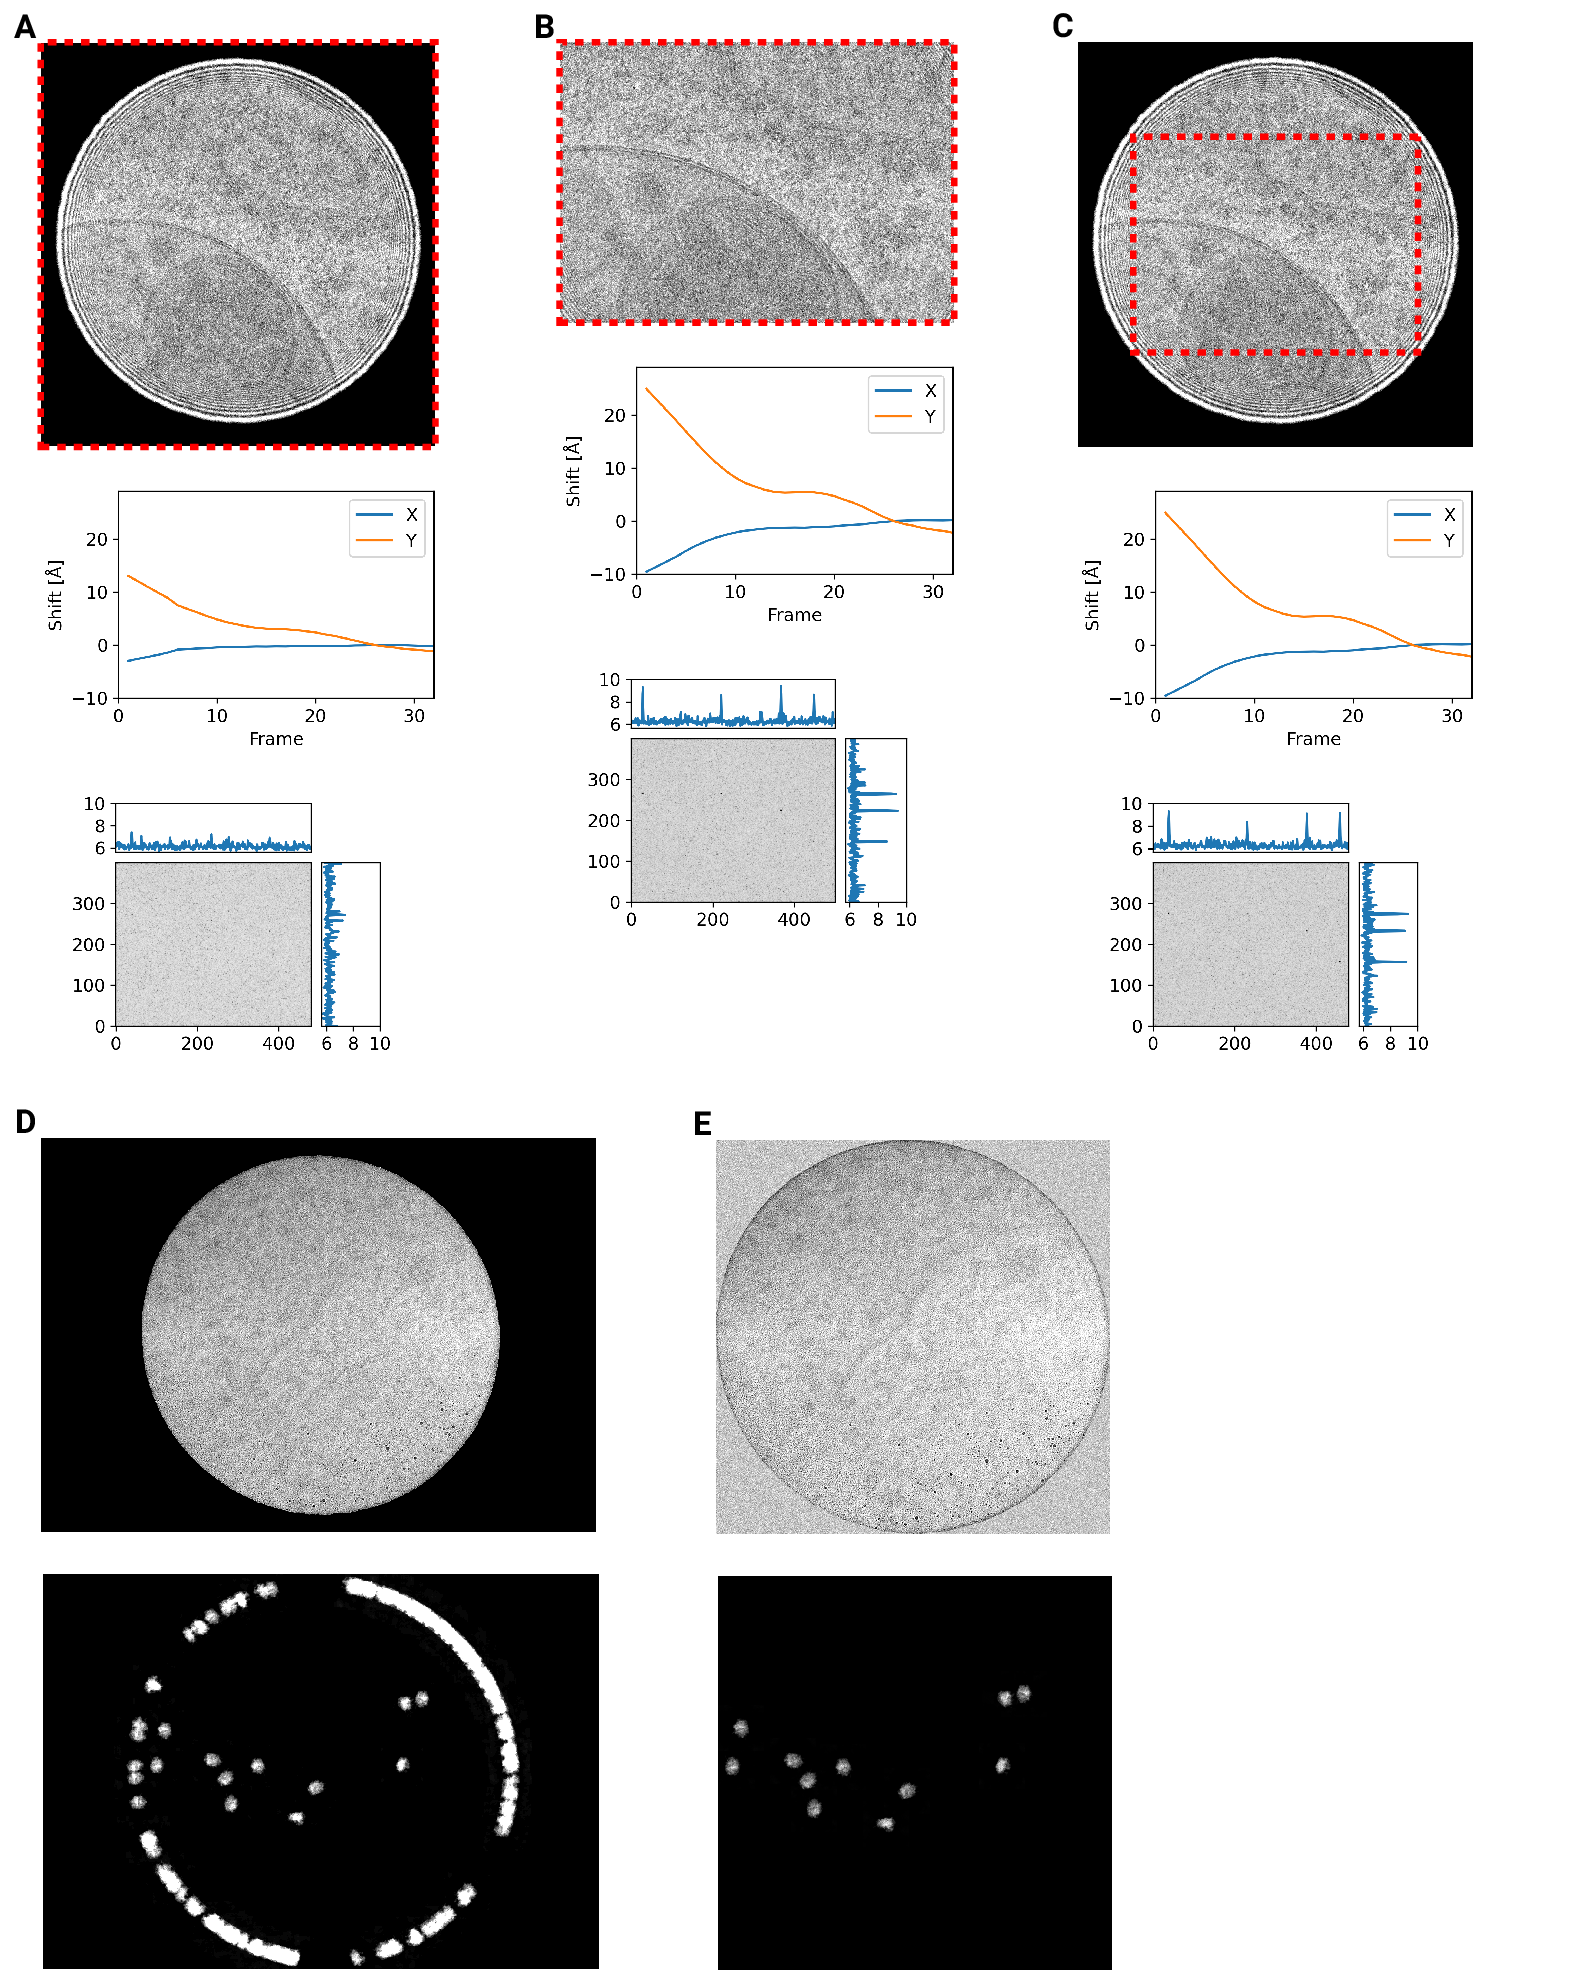
\includegraphics{figures/crop_unblur.png}
\caption{Motion correction of movies with condensed beams.
At the top of each panel is an average of the movie that was motion-corrected
with a red dashed box indicating the region that was used to estimate shifts.
Below is a graph indicating the estimated shifts of the individual frames of the
movie. Below this is the MIP of 2DTM using the large subunit of the mouse ribosome.
(A) Motion correction of the whole movie
(B) Notion correction of a cropped region of the movie that eliminates the beam
edges
(C) Motion correction of the whole movie, using only the central region to
estimate the shifts}\label{fig:crop_unblur}
}
\end{figure}

\end{fignos:tagged-figure}

\begin{fignos:tagged-figure}[4 - figure supplement 2]

\begin{figure}
\hypertarget{fig:lamella_motion_thickness}{%
\centering
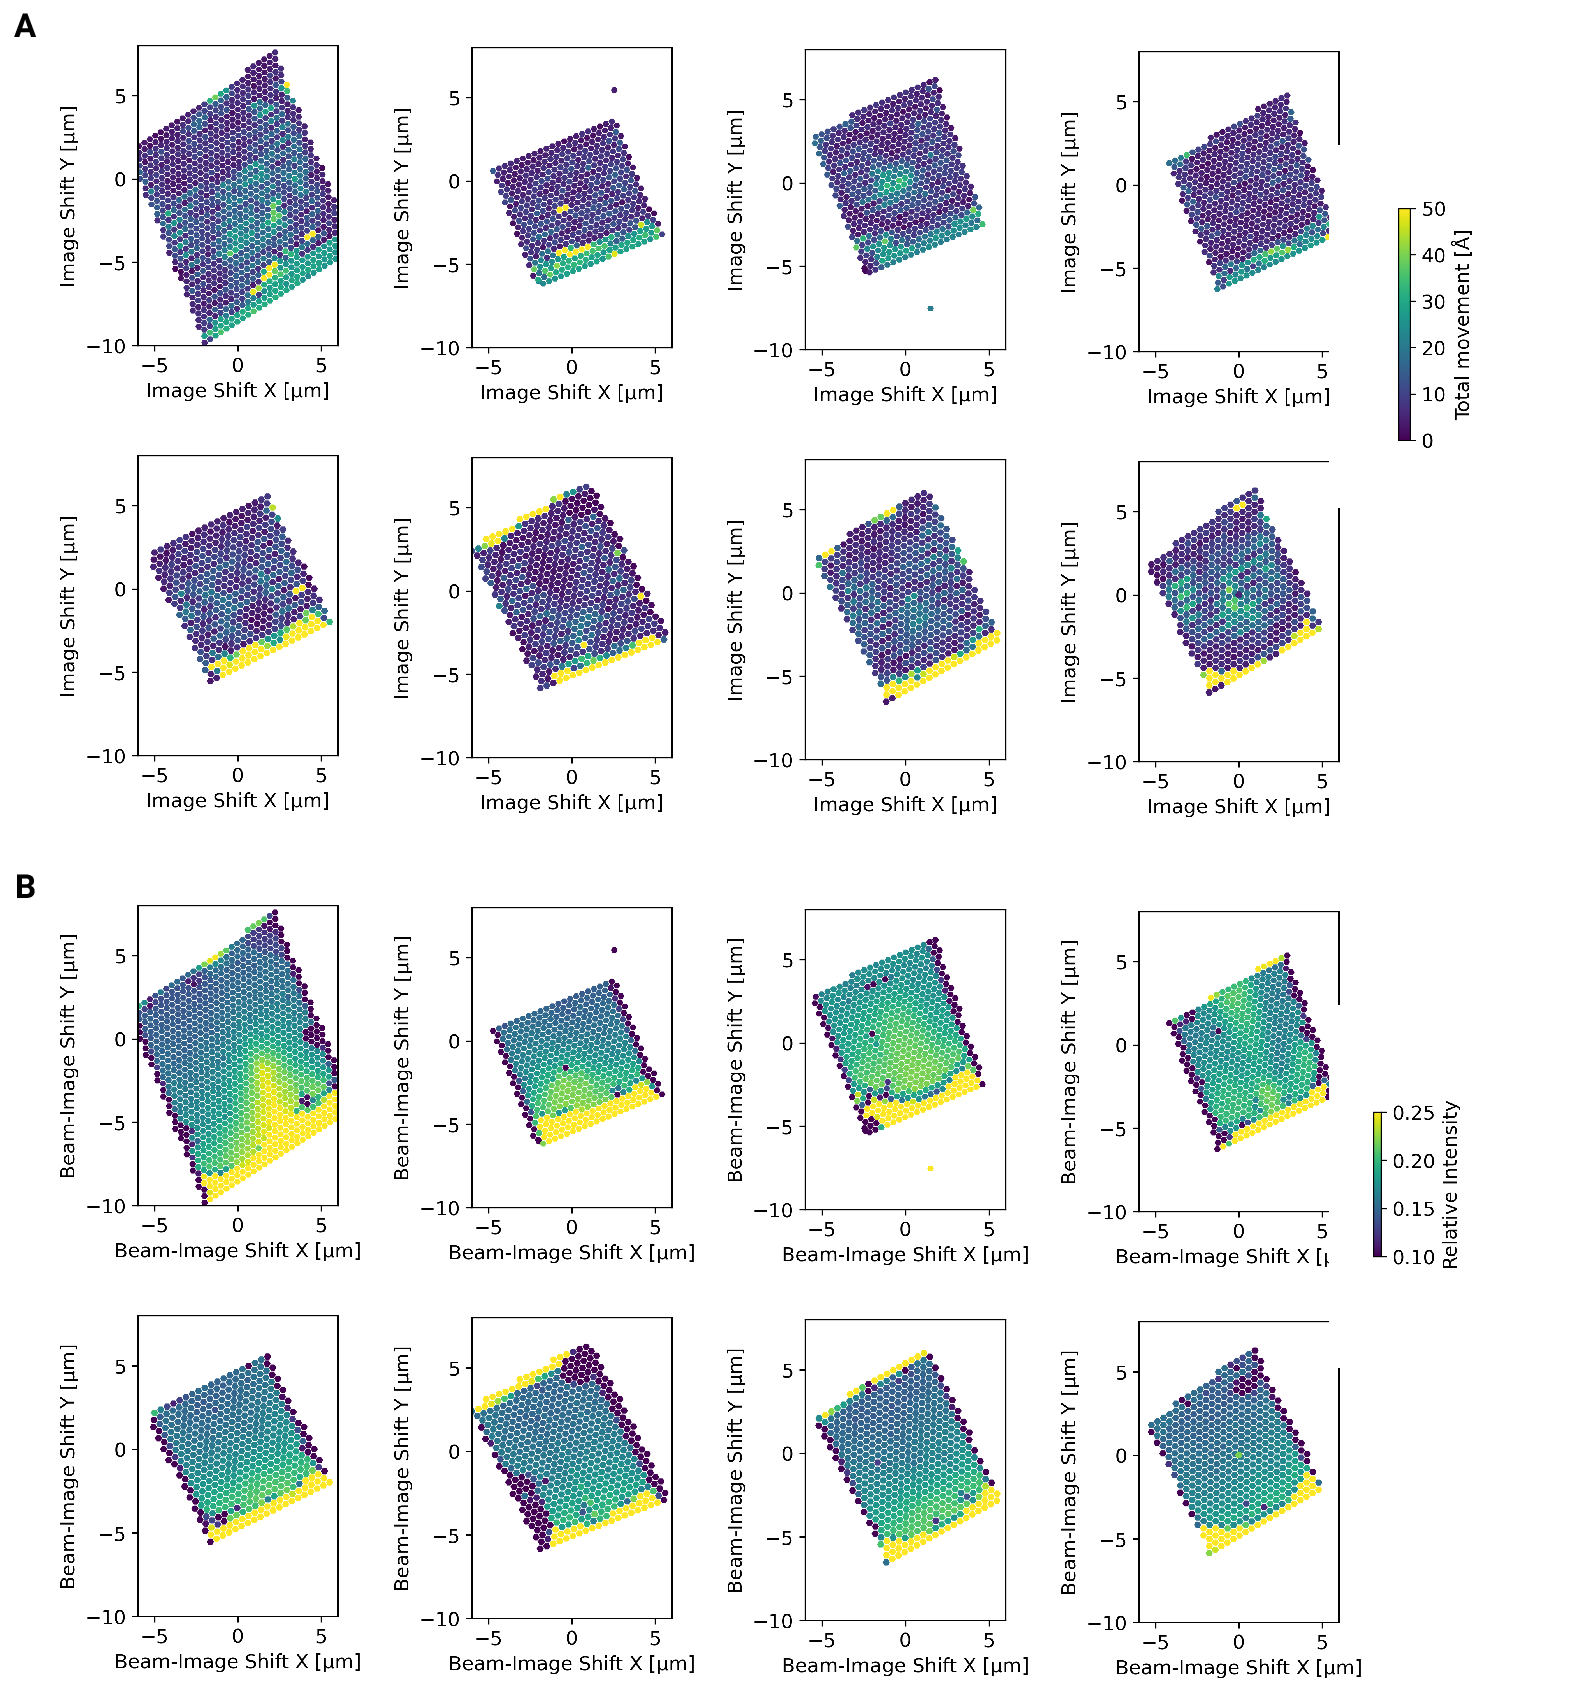
\includegraphics{figures/lamella_motion_thickness.png}
\caption{Motion correction of individual tiles imaged using the DeCo-LACE approach
(A) Total estimated motion of individual micrographs taken using the DeCo-Lace approach
plotted as a function of the beam image-shift values.
(B) Electron intensity of individual micrographs taken using the DeCo-Lace approach
plotted as a function of the beam image-shift values.}\label{fig:lamella_motion_thickness}
}
\end{figure}

\end{fignos:tagged-figure}

\begin{fignos:tagged-figure}[4 - figure supplement 3]

\begin{figure}
\hypertarget{fig:gain}{%
\centering
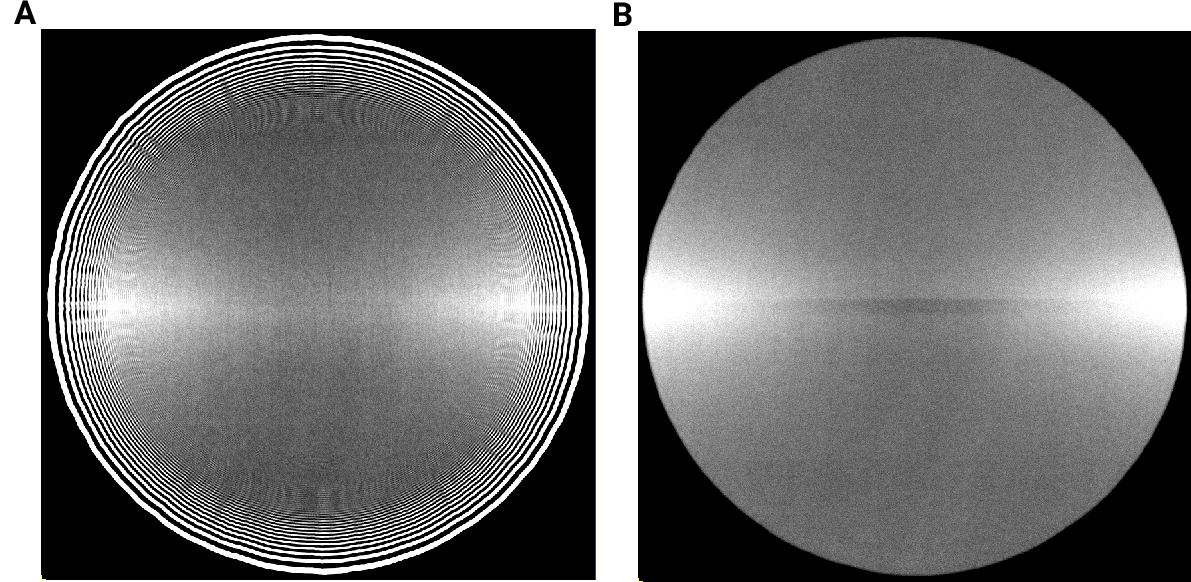
\includegraphics{figures/gain.png}
\caption{Averages of micrographs taken with a condensed beam over vacuum using a Gatan K3 detector. Contrast and Brightness have been adjusted to highlight uneven dose response. (A) Eucentric Focus (B) Fringe-free Focus}\label{fig:gain}
}
\end{figure}

\end{fignos:tagged-figure}

\begin{fignos:tagged-figure}[4 - figure supplement 4]

\begin{figure}
\hypertarget{fig:lamella_images}{%
\centering
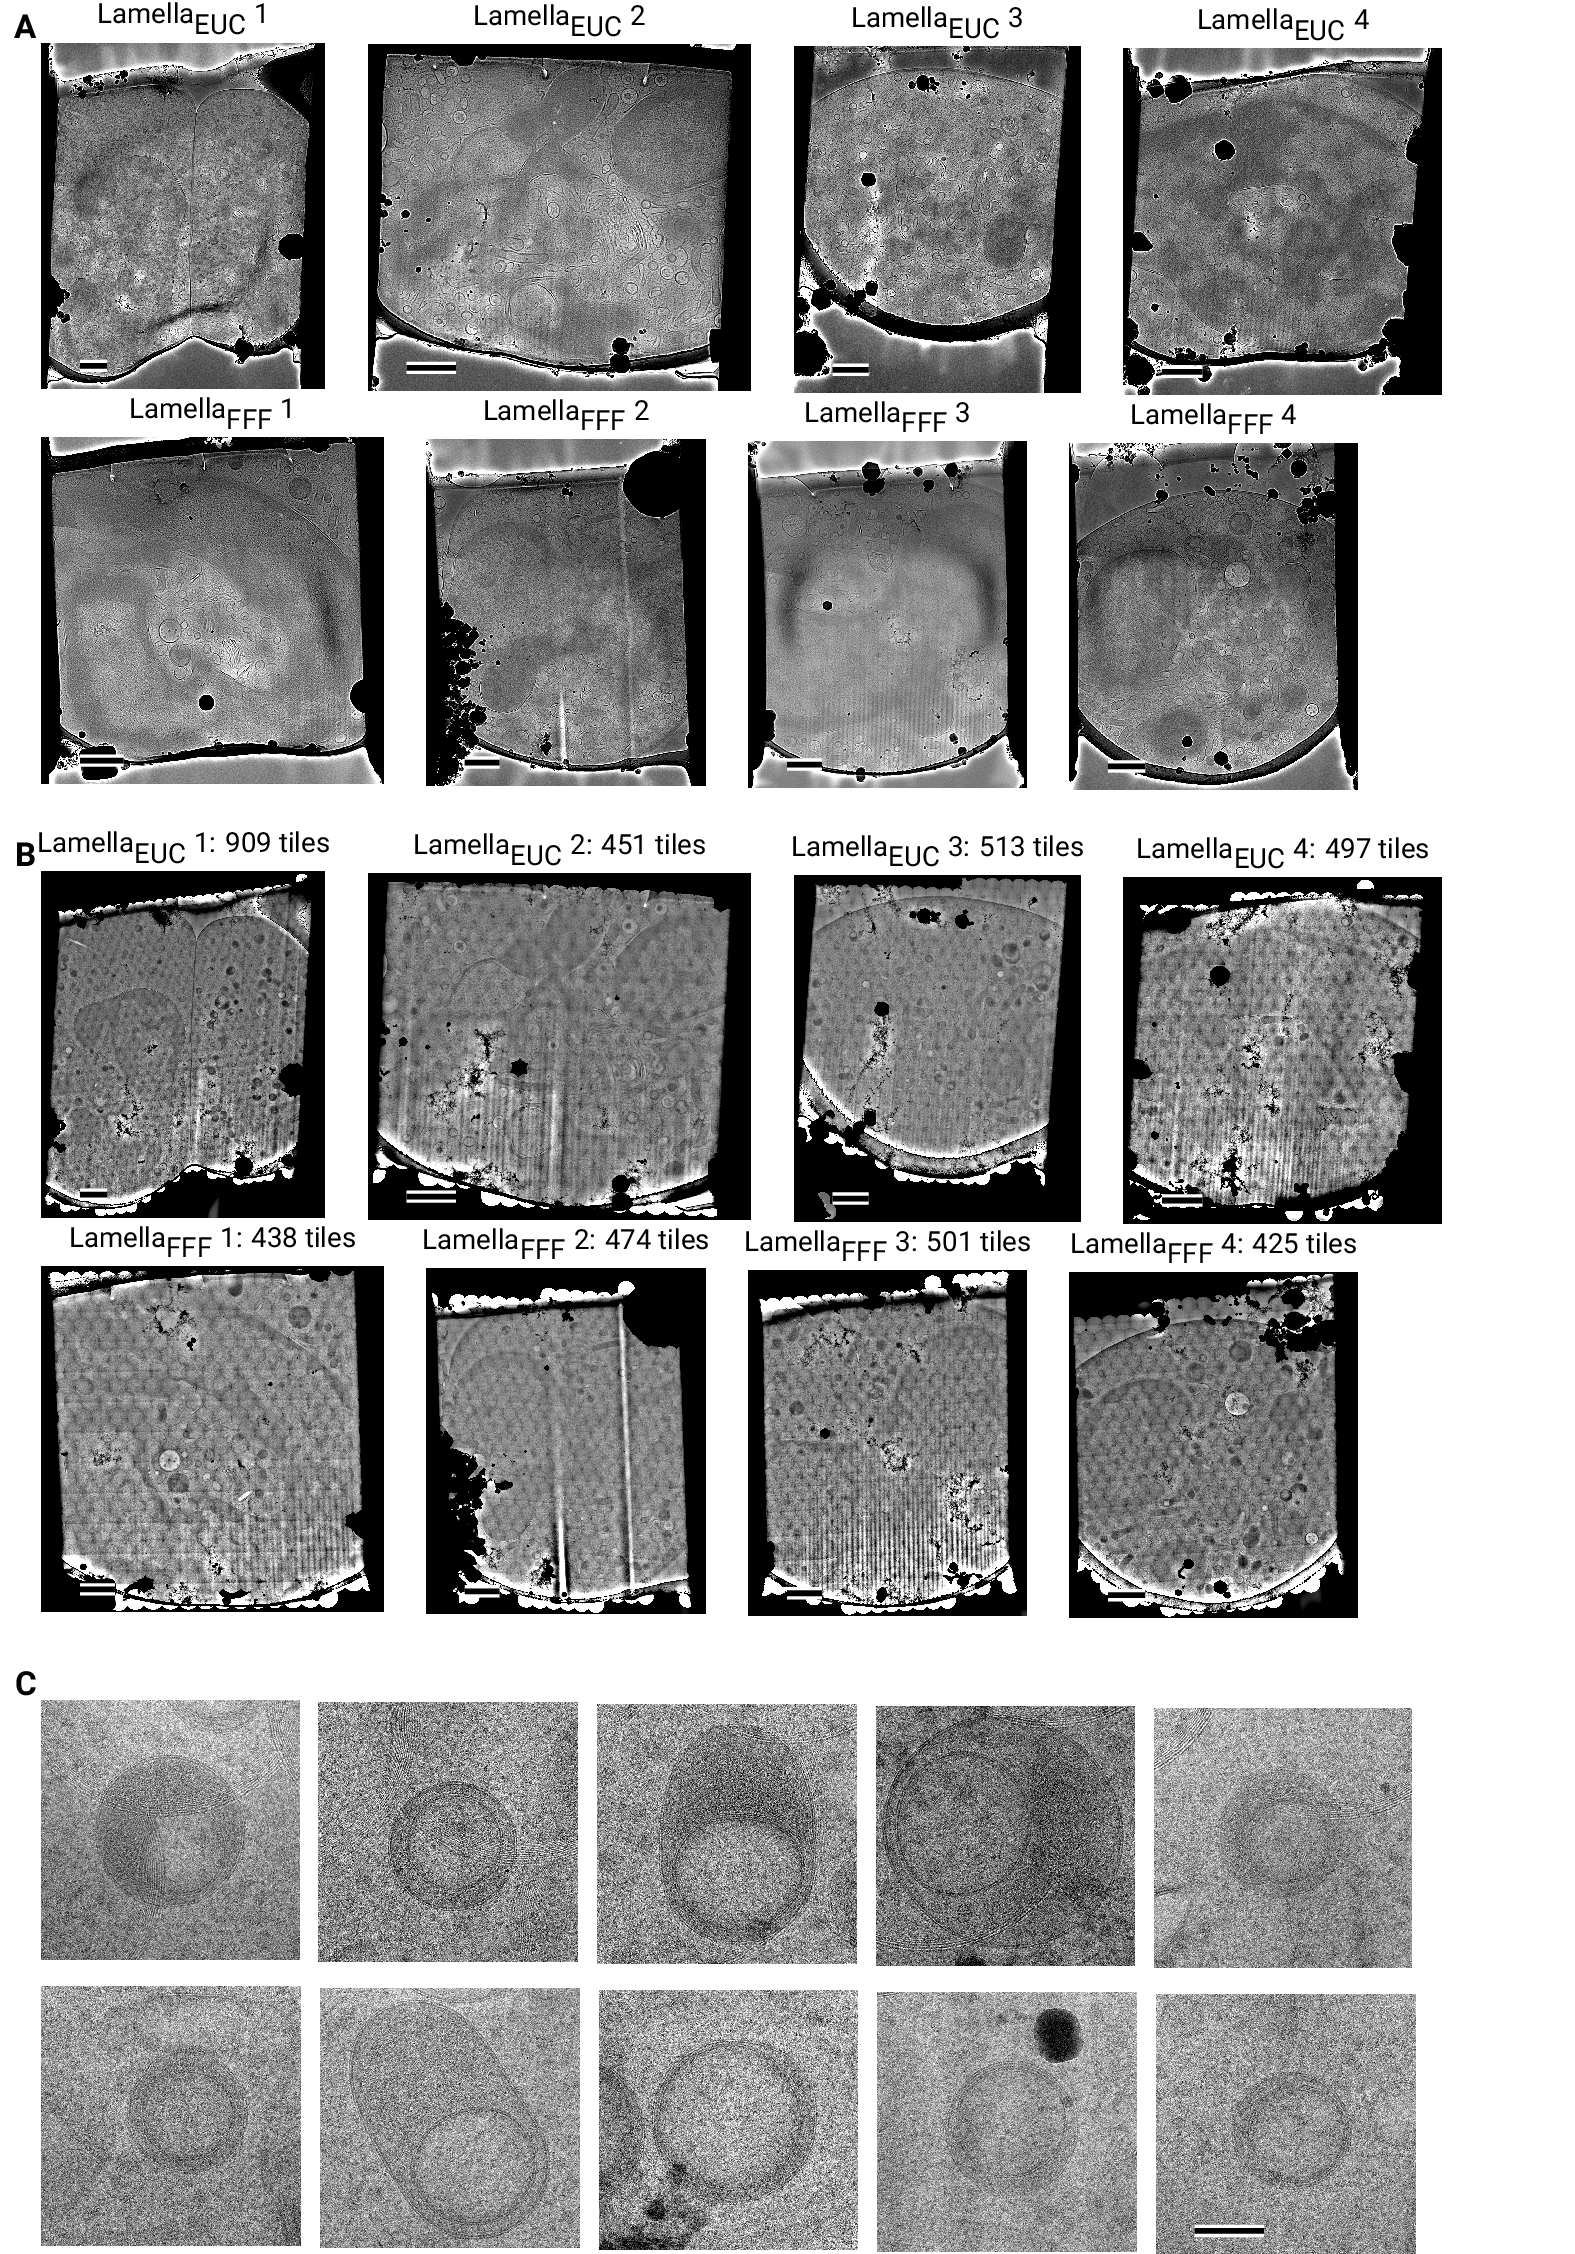
\includegraphics{figures/lamella_images.png}
\caption{Overview images of lamellae imaged using the DeCo-LACE approach taken at low-magnification (A) Overviews taken at low magnification. Scalebar corresponds to 1 μm. (B) Overviews assembled using the DeCo-LACE approach. Scalebar corresponds to 1 μm. (C) Representative examples of a class of granules containing a putatively cytosolic inclusion. Scalebar corresponds to 100 nm.}\label{fig:lamella_images}
}
\end{figure}

\end{fignos:tagged-figure}

\begin{figure}
\hypertarget{fig:matching_stat}{%
\centering
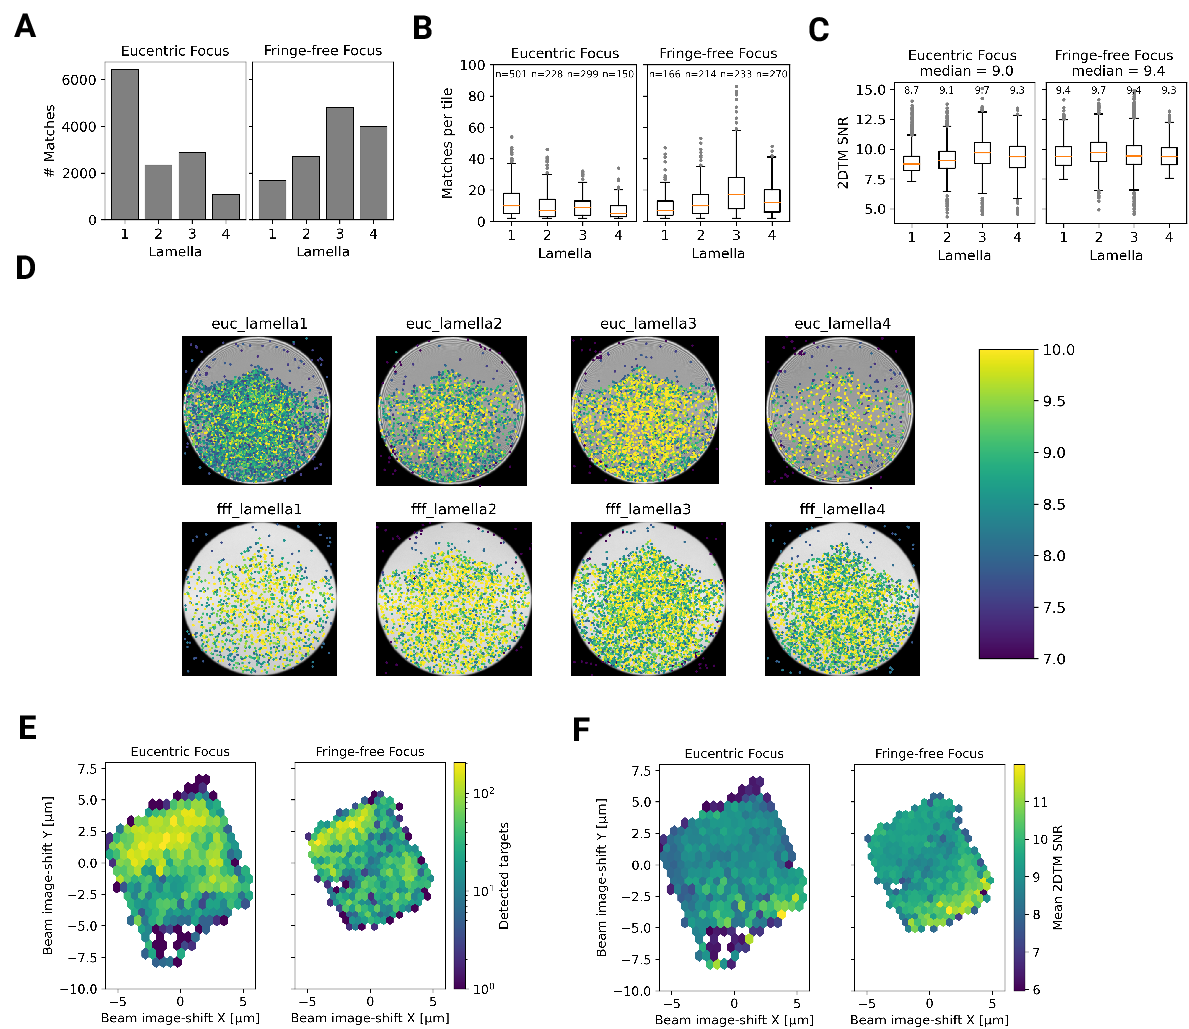
\includegraphics{figures/matching_stat.png}
\caption{Statistics of 2DTM on lamella imaged using DeCo-LACE (A) Number of detected targets in
each lamella (B) Distribution of targets per tile in each lamella. Only tiles
with two or more detected targets were included (C) Distribution of SNRs in each lamella
(D) For each lamella an average of all tiles is shown. Overlaid is a scatterplot
of all detected targets in these tiles according to their in-tile coordinates.
Scatterplot is colored according to the 2DTM SNR. There are no detected targets in the top
circle-circle intersection due to radiation damage from previous exposures. (E) 2D histogram of number of detected targets as a function of beam-image shift (F) Mean 2DTM SNR as a function of beam-image shift}\label{fig:matching_stat}
}
\end{figure}

\begin{figure}
\hypertarget{fig:matching_euc}{%
\centering
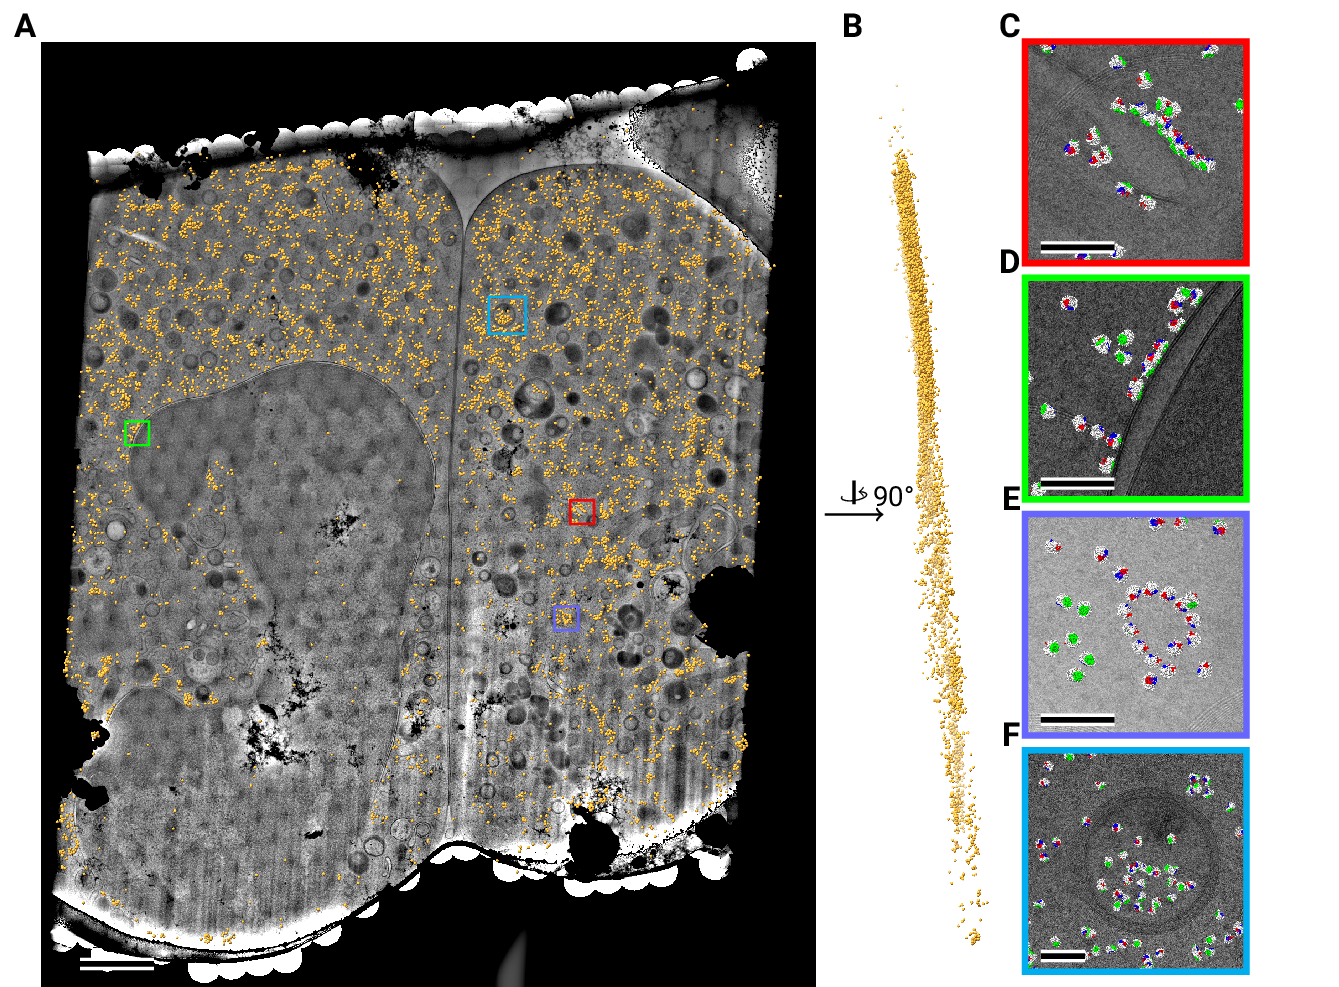
\includegraphics{figures/matching_euc.png}
\caption{Template matching in lamella imaged using the DeCo-Lace approach at eucentric
focus (A) Montage of Lamella\(_\textrm{EUC}\) 1 overlaid with detected targets according to
their montage coordinates colored in orange. Scalebar corresponds to 1 μm. (B) Side view of detected targets in the lamella, such that the
direction of the electron beam is horizontal. (C-F) Magnified area of panel A
showing rough ER with associated ribosomes(C), outer nuclear membrane with
associated ribosomes (D), ribsomes arranged in a circular fashion(E), ribosomes
enclosed in a less electron dense inclusion in a granule(F). Ribosomes are colored in white with the surface of the peptide exit tunnel colored in green and the A, P, and E sites colored in blue, purple, and red, respectively.Scalebar corresponds to 100 nm.}\label{fig:matching_euc}
}
\end{figure}

\begin{figure}
\hypertarget{fig:matching_fff}{%
\centering
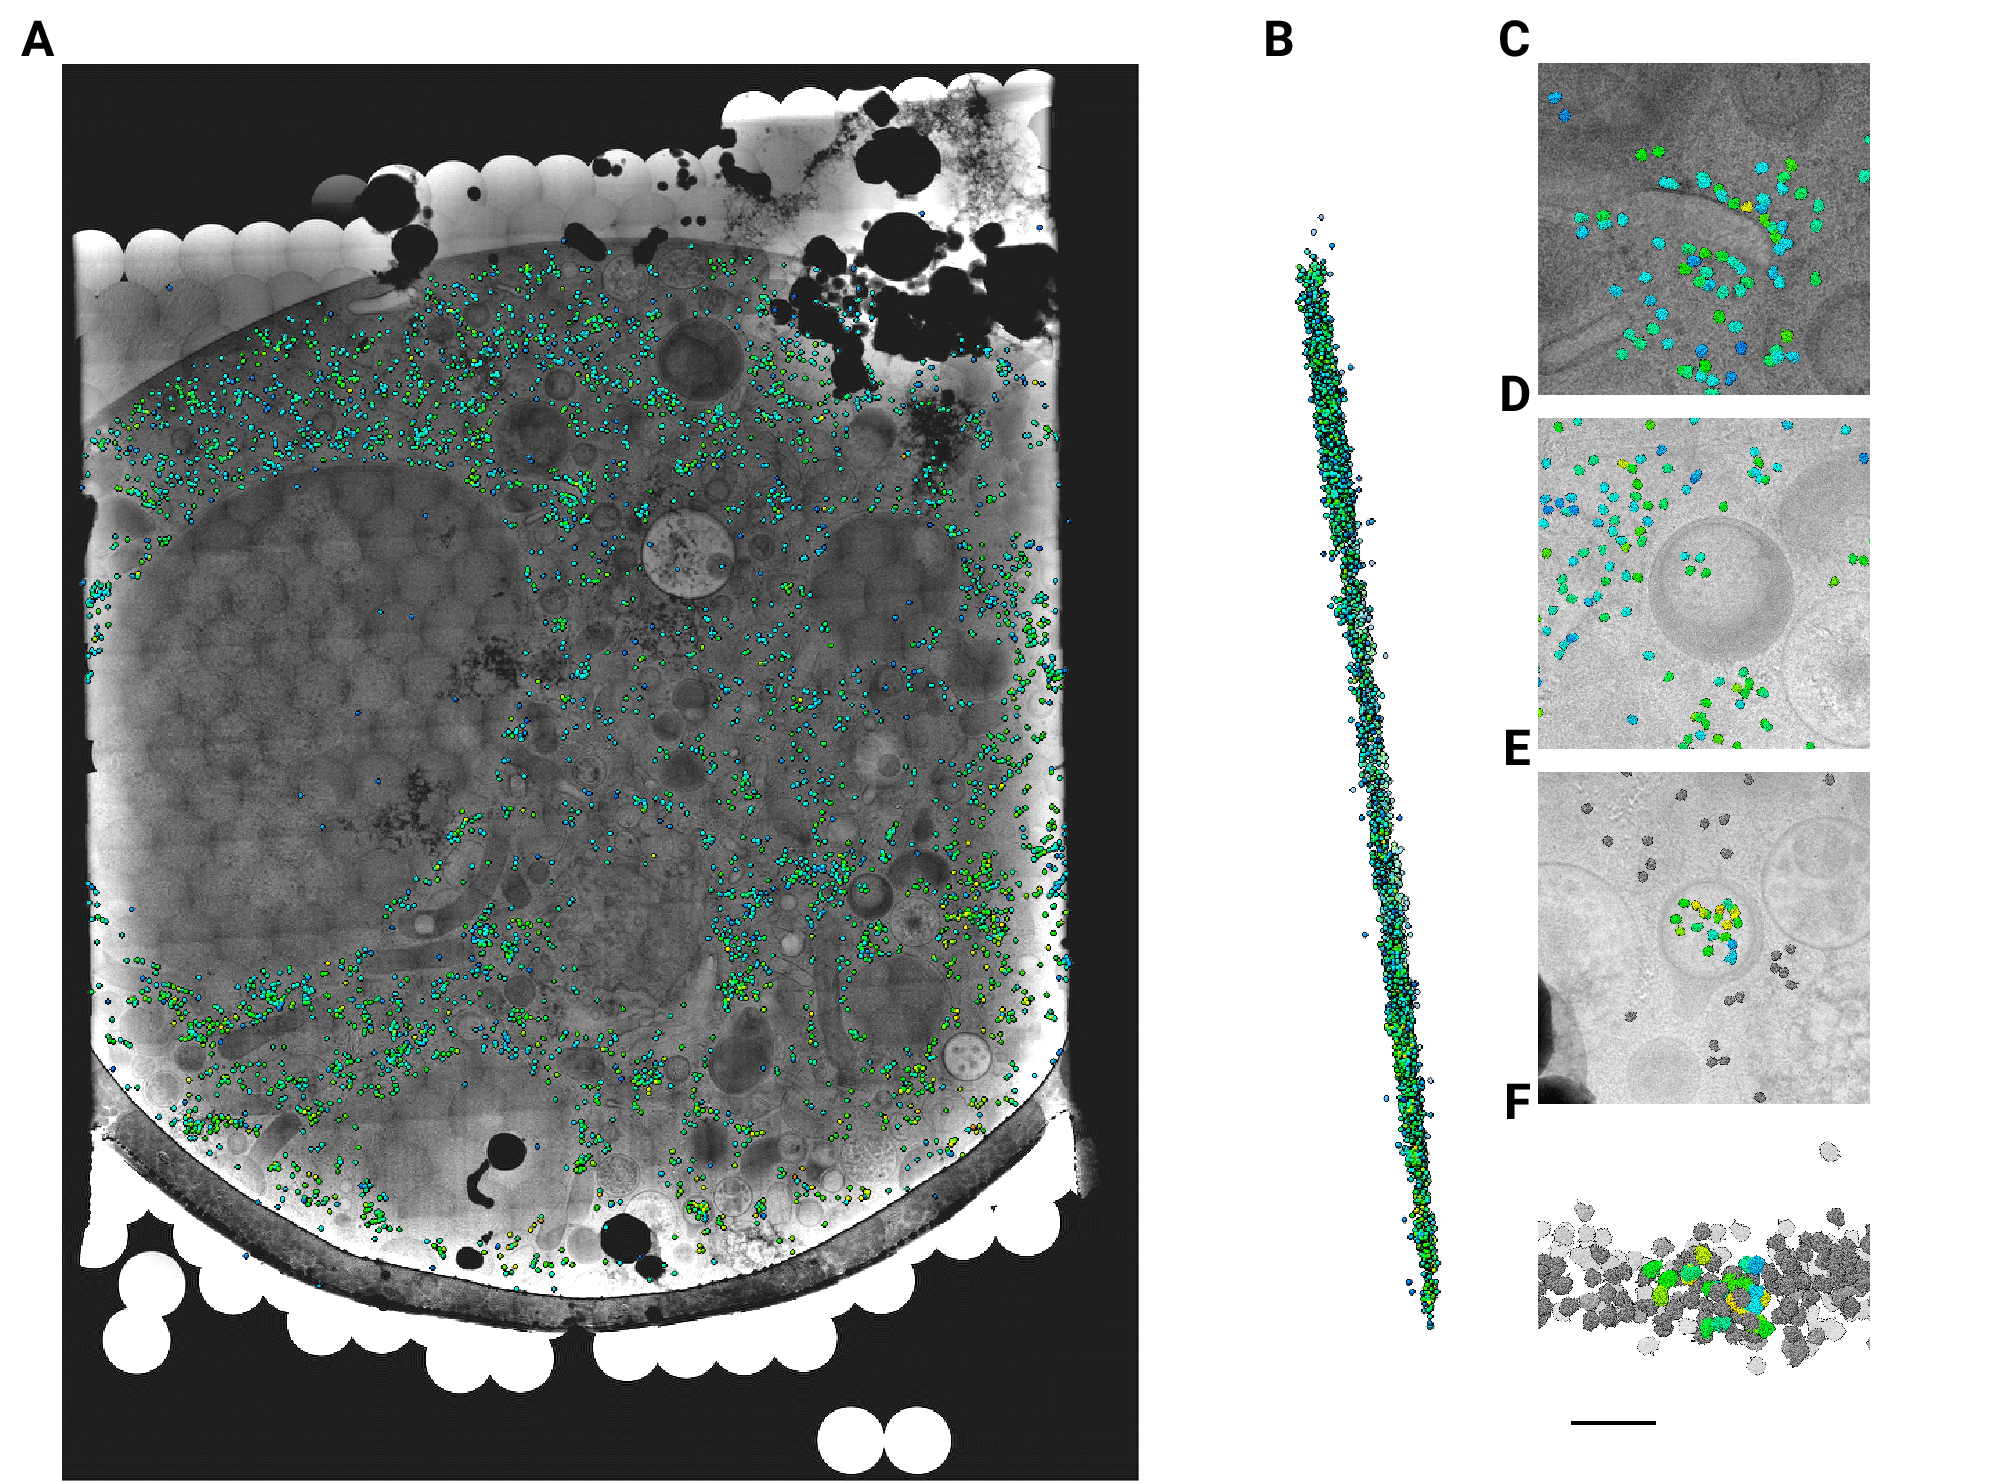
\includegraphics{figures/matching_fff.png}
\caption{Template matching in lamella imaged using the DeCo-Lace approach at fringe-free
focus (A) Montage of Lamella\(_\textrm{FFF}\) 4 overlaid with detected targets according to
their montage coordinates colored in orange. Scalebar corresponds to 1 μm. (B) Side view of detected targets in the lamella, such that the
direction of the electron beam is horizontal. (C-E) Magnified area of panel A
showing rough ER with associated ribosomes(C) and ribosomes
enclosed in a less electron dense inclusion in a granule(D,E). (F) Side view of
panel E. Ribosomes are colored in white with the surface of the peptide exit tunnel colored in green and the A, P, and E sites colored in blue, purple, and red, respectively. Scalebar corresponds to 100 nm.}\label{fig:matching_fff}
}
\end{figure}

\hypertarget{references}{%
\subsection{References}\label{references}}

\hypertarget{refs}{}
\begin{CSLReferences}{0}{0}
\leavevmode\vadjust pre{\hypertarget{ref-tSXIKPl7}{}}%
\CSLLeftMargin{1. }%
\CSLRightInline{\textbf{Label-free, normalized quantification of complex mass spectrometry data for proteomic analysis}
\CSLBlock{Noelle M Griffin, Jingyi Yu, Fred Long, Phil Oh, Sabrina Shore, Yan Li, Jim A Koziol, Jan E Schnitzer} \emph{Nature Biotechnology} (2010-01) \url{https://doi.org/fshgnc}
\CSLBlock{DOI: \href{https://doi.org/10.1038/nbt.1592}{10.1038/nbt.1592} · PMID: \href{https://www.ncbi.nlm.nih.gov/pubmed/20010810}{20010810} · PMCID: \href{https://www.ncbi.nlm.nih.gov/pmc/articles/PMC2805705}{PMC2805705}}}

\leavevmode\vadjust pre{\hypertarget{ref-VBmW7Aot}{}}%
\CSLLeftMargin{2. }%
\CSLRightInline{\textbf{Fluorescence microscopy}
\CSLBlock{Jeff W Lichtman, José-Angel Conchello} \emph{Nature Methods} (2005-11-18) \url{https://doi.org/bbpg4n}
\CSLBlock{DOI: \href{https://doi.org/10.1038/nmeth817}{10.1038/nmeth817} · PMID: \href{https://www.ncbi.nlm.nih.gov/pubmed/16299476}{16299476}}}

\leavevmode\vadjust pre{\hypertarget{ref-tGQ6TSUo}{}}%
\CSLLeftMargin{3. }%
\CSLRightInline{\textbf{A visual approach to proteomics}
\CSLBlock{Stephan Nickell, Christine Kofler, Andrew P Leis, Wolfgang Baumeister} \emph{Nature Reviews Molecular Cell Biology} (2006-02-15) \url{https://doi.org/d6d5mq}
\CSLBlock{DOI: \href{https://doi.org/10.1038/nrm1861}{10.1038/nrm1861} · PMID: \href{https://www.ncbi.nlm.nih.gov/pubmed/16482091}{16482091}}}

\leavevmode\vadjust pre{\hypertarget{ref-g8QavfwP}{}}%
\CSLLeftMargin{4. }%
\CSLRightInline{\textbf{Electron microscopy of frozen hydrated sections of vitreous ice and vitrified biological samples}
\CSLBlock{AW McDowall, J-J Chang, R Freeman, J Lepault, CA Walter, J Dubochet} \emph{Journal of Microscopy} (1983-07) \url{https://doi.org/bdnzmv}
\CSLBlock{DOI: \href{https://doi.org/10.1111/j.1365-2818.1983.tb04225.x}{10.1111/j.1365-2818.1983.tb04225.x} · PMID: \href{https://www.ncbi.nlm.nih.gov/pubmed/6350598}{6350598}}}

\leavevmode\vadjust pre{\hypertarget{ref-16IhS1Nc4}{}}%
\CSLLeftMargin{5. }%
\CSLRightInline{\textbf{Opening windows into the cell: focused-ion-beam milling for cryo-electron tomography}
\CSLBlock{Elizabeth Villa, Miroslava Schaffer, Jürgen M Plitzko, Wolfgang Baumeister} \emph{Current Opinion in Structural Biology} (2013-10) \url{https://doi.org/f537jp}
\CSLBlock{DOI: \href{https://doi.org/10.1016/j.sbi.2013.08.006}{10.1016/j.sbi.2013.08.006} · PMID: \href{https://www.ncbi.nlm.nih.gov/pubmed/24090931}{24090931}}}

\leavevmode\vadjust pre{\hypertarget{ref-Rksh2dxu}{}}%
\CSLLeftMargin{6. }%
\CSLRightInline{\textbf{Electron tomography of cells}
\CSLBlock{Lu Gan, Grant J Jensen} \emph{Quarterly Reviews of Biophysics} (2011-11-15) \url{https://doi.org/czj9hr}
\CSLBlock{DOI: \href{https://doi.org/10.1017/s0033583511000102}{10.1017/s0033583511000102} · PMID: \href{https://www.ncbi.nlm.nih.gov/pubmed/22082691}{22082691}}}

\leavevmode\vadjust pre{\hypertarget{ref-Ynb3IP6I}{}}%
\CSLLeftMargin{7. }%
\CSLRightInline{\textbf{Single-protein detection in crowded molecular environments in cryo-EM images}
\CSLBlock{JPeter Rickgauer, Nikolaus Grigorieff, Winfried Denk} \emph{eLife} (2017-05-03) \url{https://doi.org/gnq4q4}
\CSLBlock{DOI: \href{https://doi.org/10.7554/elife.25648}{10.7554/elife.25648} · PMID: \href{https://www.ncbi.nlm.nih.gov/pubmed/28467302}{28467302} · PMCID: \href{https://www.ncbi.nlm.nih.gov/pmc/articles/PMC5453696}{PMC5453696}}}

\leavevmode\vadjust pre{\hypertarget{ref-18KGpXYPE}{}}%
\CSLLeftMargin{8. }%
\CSLRightInline{\textbf{Label-free single-instance protein detection in vitrified cells}
\CSLBlock{JPeter Rickgauer, Heejun Choi, Jennifer Lippincott-Schwartz, Winfried Denk} \emph{Cold Spring Harbor Laboratory} (2020-04-24) \url{https://doi.org/gpbjfd}
\CSLBlock{DOI: \href{https://doi.org/10.1101/2020.04.22.053868}{10.1101/2020.04.22.053868}}}

\leavevmode\vadjust pre{\hypertarget{ref-10bXZuF3G}{}}%
\CSLLeftMargin{9. }%
\CSLRightInline{\textbf{Locating macromolecular assemblies in cells by 2D template matching with cisTEM}
\CSLBlock{Bronwyn A Lucas, Benjamin A Himes, Liang Xue, Timothy Grant, Julia Mahamid, Nikolaus Grigorieff} \emph{eLife} (2021-06-11) \url{https://doi.org/gkkc49}
\CSLBlock{DOI: \href{https://doi.org/10.7554/elife.68946}{10.7554/elife.68946} · PMID: \href{https://www.ncbi.nlm.nih.gov/pubmed/34114559}{34114559} · PMCID: \href{https://www.ncbi.nlm.nih.gov/pmc/articles/PMC8219381}{PMC8219381}}}

\leavevmode\vadjust pre{\hypertarget{ref-1B9Vt9eYu}{}}%
\CSLLeftMargin{10. }%
\CSLRightInline{\textbf{Inhibition of Dihydroorotate Dehydrogenase Overcomes Differentiation Blockade in Acute Myeloid Leukemia}
\CSLBlock{David B Sykes, Youmna S Kfoury, François E Mercier, Mathias J Wawer, Jason M Law, Mark K Haynes, Timothy A Lewis, Amir Schajnovitz, Esha Jain, Dongjun Lee, \ldots{} David T Scadden} \emph{Cell} (2016-09) \url{https://doi.org/f3r5jr}
\CSLBlock{DOI: \href{https://doi.org/10.1016/j.cell.2016.08.057}{10.1016/j.cell.2016.08.057} · PMID: \href{https://www.ncbi.nlm.nih.gov/pubmed/27641501}{27641501} · PMCID: \href{https://www.ncbi.nlm.nih.gov/pmc/articles/PMC7360335}{PMC7360335}}}

\leavevmode\vadjust pre{\hypertarget{ref-gRoY21jY}{}}%
\CSLLeftMargin{11. }%
\CSLRightInline{\textbf{Hallmarks of ribosomopathies}
\CSLBlock{Kim R Kampen, Sergey O Sulima, Stijn Vereecke, Kim De~Keersmaecker} \emph{Nucleic Acids Research} (2019-07-27) \url{https://doi.org/gpbjfm}
\CSLBlock{DOI: \href{https://doi.org/10.1093/nar/gkz637}{10.1093/nar/gkz637} · PMID: \href{https://www.ncbi.nlm.nih.gov/pubmed/31350888}{31350888} · PMCID: \href{https://www.ncbi.nlm.nih.gov/pmc/articles/PMC7026650}{PMC7026650}}}

\leavevmode\vadjust pre{\hypertarget{ref-KAJ7221k}{}}%
\CSLLeftMargin{12. }%
\CSLRightInline{\textbf{Diagnostic and prognostic implications of ribosomal protein transcript expression patterns in human cancers}
\CSLBlock{James M Dolezal, Arie P Dash, Edward V Prochownik} \emph{BMC Cancer} (2018-03-12) \url{https://doi.org/gc87j9}
\CSLBlock{DOI: \href{https://doi.org/10.1186/s12885-018-4178-z}{10.1186/s12885-018-4178-z} · PMID: \href{https://www.ncbi.nlm.nih.gov/pubmed/29530001}{29530001} · PMCID: \href{https://www.ncbi.nlm.nih.gov/pmc/articles/PMC5848553}{PMC5848553}}}

\leavevmode\vadjust pre{\hypertarget{ref-19ZFerhph}{}}%
\CSLLeftMargin{13. }%
\CSLRightInline{\textbf{Automated electron microscope tomography using robust prediction of specimen movements}
\CSLBlock{David N Mastronarde} \emph{Journal of Structural Biology} (2005-10) \url{https://doi.org/ff7gzx}
\CSLBlock{DOI: \href{https://doi.org/10.1016/j.jsb.2005.07.007}{10.1016/j.jsb.2005.07.007} · PMID: \href{https://www.ncbi.nlm.nih.gov/pubmed/16182563}{16182563}}}

\leavevmode\vadjust pre{\hypertarget{ref-MUY42yxp}{}}%
\CSLLeftMargin{14. }%
\CSLRightInline{\textbf{cisTEM, user-friendly software for single-particle image processing}
\CSLBlock{Timothy Grant, Alexis Rohou, Nikolaus Grigorieff} \emph{eLife} (2018-03-07) \url{https://doi.org/gf5cq7}
\CSLBlock{DOI: \href{https://doi.org/10.7554/elife.35383}{10.7554/elife.35383} · PMID: \href{https://www.ncbi.nlm.nih.gov/pubmed/29513216}{29513216} · PMCID: \href{https://www.ncbi.nlm.nih.gov/pmc/articles/PMC5854467}{PMC5854467}}}

\leavevmode\vadjust pre{\hypertarget{ref-1G4Y94qCy}{}}%
\CSLLeftMargin{15. }%
\CSLRightInline{\textbf{Measuring the optimal exposure for single particle cryo-EM using a 2.6 Å reconstruction of rotavirus VP6}
\CSLBlock{Timothy Grant, Nikolaus Grigorieff} \emph{eLife} (2015-05-29) \url{https://doi.org/gf5cm7}
\CSLBlock{DOI: \href{https://doi.org/10.7554/elife.06980}{10.7554/elife.06980} · PMID: \href{https://www.ncbi.nlm.nih.gov/pubmed/26023829}{26023829} · PMCID: \href{https://www.ncbi.nlm.nih.gov/pmc/articles/PMC4471936}{PMC4471936}}}

\leavevmode\vadjust pre{\hypertarget{ref-n43f3Sqs}{}}%
\CSLLeftMargin{16. }%
\CSLRightInline{\textbf{CTFFIND4: Fast and accurate defocus estimation from electron micrographs}
\CSLBlock{Alexis Rohou, Nikolaus Grigorieff} \emph{Journal of Structural Biology} (2015-11) \url{https://doi.org/f7xzgv}
\CSLBlock{DOI: \href{https://doi.org/10.1016/j.jsb.2015.08.008}{10.1016/j.jsb.2015.08.008} · PMID: \href{https://www.ncbi.nlm.nih.gov/pubmed/26278980}{26278980} · PMCID: \href{https://www.ncbi.nlm.nih.gov/pmc/articles/PMC6760662}{PMC6760662}}}

\leavevmode\vadjust pre{\hypertarget{ref-q2PSamkS}{}}%
\CSLLeftMargin{17. }%
\CSLRightInline{\textbf{Cryo-TEM simulations of amorphous radiation-sensitive samples using multislice wave propagation}
\CSLBlock{Benjamin Himes, Nikolaus Grigorieff} \emph{IUCrJ} (2021-09-30) \url{https://doi.org/gpzs9r}
\CSLBlock{DOI: \href{https://doi.org/10.1107/s2052252521008538}{10.1107/s2052252521008538} · PMID: \href{https://www.ncbi.nlm.nih.gov/pubmed/34804546}{34804546} · PMCID: \href{https://www.ncbi.nlm.nih.gov/pmc/articles/PMC8562658}{PMC8562658}}}

\leavevmode\vadjust pre{\hypertarget{ref-stvWEJeu}{}}%
\CSLLeftMargin{18. }%
\CSLRightInline{\textbf{scikit-image: image processing in Python}
\CSLBlock{Stéfan van der Walt, Johannes L Schönberger, Juan Nunez-Iglesias, François Boulogne, Joshua D Warner, Neil Yager, Emmanuelle Gouillart, Tony Yu} \emph{PeerJ} (2014-06-19) \url{https://doi.org/gftp3s}
\CSLBlock{DOI: \href{https://doi.org/10.7717/peerj.453}{10.7717/peerj.453} · PMID: \href{https://www.ncbi.nlm.nih.gov/pubmed/25024921}{25024921} · PMCID: \href{https://www.ncbi.nlm.nih.gov/pmc/articles/PMC4081273}{PMC4081273}}}

\leavevmode\vadjust pre{\hypertarget{ref-8Miti2Gz}{}}%
\CSLLeftMargin{19. }%
\CSLRightInline{\textbf{SciPy 1.0: fundamental algorithms for scientific computing in Python}
\CSLBlock{Pauli Virtanen, Ralf Gommers, Travis E Oliphant, Matt Haberland, Tyler Reddy, David Cournapeau, Evgeni Burovski, Pearu Peterson, Warren Weckesser, Jonathan Bright, \ldots{} } \emph{Nature Methods} (2020-02-03) \url{https://doi.org/ggj45f}
\CSLBlock{DOI: \href{https://doi.org/10.1038/s41592-019-0686-2}{10.1038/s41592-019-0686-2} · PMID: \href{https://www.ncbi.nlm.nih.gov/pubmed/32015543}{32015543} · PMCID: \href{https://www.ncbi.nlm.nih.gov/pmc/articles/PMC7056644}{PMC7056644}}}

\leavevmode\vadjust pre{\hypertarget{ref-cYCuuZxG}{}}%
\CSLLeftMargin{20. }%
\CSLRightInline{\textbf{\textless scp\textgreater UCSF ChimeraX\textless/scp\textgreater{}
: Structure visualization for researchers, educators, and developers}
\CSLBlock{Eric F Pettersen, Thomas D Goddard, Conrad C Huang, Elaine C Meng, Gregory S Couch, Tristan I Croll, John H Morris, Thomas E Ferrin} \emph{Protein Science} (2020-10-22) \url{https://doi.org/ghr6mn}
\CSLBlock{DOI: \href{https://doi.org/10.1002/pro.3943}{10.1002/pro.3943} · PMID: \href{https://www.ncbi.nlm.nih.gov/pubmed/32881101}{32881101} · PMCID: \href{https://www.ncbi.nlm.nih.gov/pmc/articles/PMC7737788}{PMC7737788}}}

\leavevmode\vadjust pre{\hypertarget{ref-sbkam02a}{}}%
\CSLLeftMargin{21. }%
\CSLRightInline{\textbf{Protein Synthesis in the Developing Neocortex at Near-Atomic Resolution Reveals Ebp1-Mediated Neuronal Proteostasis at the 60S Tunnel Exit}
\CSLBlock{Matthew L Kraushar, Ferdinand Krupp, Dermot Harnett, Paul Turko, Mateusz C Ambrozkiewicz, Thiemo Sprink, Koshi Imami, Manuel Günnigmann, Ulrike Zinnall, Carlos H Vieira-Vieira, \ldots{} Christian MT Spahn} \emph{Molecular Cell} (2021-01) \url{https://doi.org/gh7d72}
\CSLBlock{DOI: \href{https://doi.org/10.1016/j.molcel.2020.11.037}{10.1016/j.molcel.2020.11.037} · PMID: \href{https://www.ncbi.nlm.nih.gov/pubmed/33357414}{33357414} · PMCID: \href{https://www.ncbi.nlm.nih.gov/pmc/articles/PMC8163098}{PMC8163098}}}

\leavevmode\vadjust pre{\hypertarget{ref-APSL9LmU}{}}%
\CSLLeftMargin{22. }%
\CSLRightInline{\textbf{High-quality, high-throughput cryo-electron microscopy data collection via beam tilt and astigmatism-free beam-image shift}
\CSLBlock{Chunling Wu, Xiaojun Huang, Jing Cheng, Dongjie Zhu, Xinzheng Zhang} \emph{Journal of Structural Biology} (2019-12) \url{https://doi.org/gp2nq9}
\CSLBlock{DOI: \href{https://doi.org/10.1016/j.jsb.2019.09.013}{10.1016/j.jsb.2019.09.013} · PMID: \href{https://www.ncbi.nlm.nih.gov/pubmed/31562921}{31562921}}}

\leavevmode\vadjust pre{\hypertarget{ref-xE2EhAcH}{}}%
\CSLLeftMargin{23. }%
\CSLRightInline{\textbf{THE DEVELOPMENT OF NEUTROPHILIC POLYMORPHONUCLEAR LEUKOCYTES IN HUMAN BONE MARROW}
\CSLBlock{Dorothy Ford Bainton, Joan L Ullyot, Marilyn G Farquhar} \emph{Journal of Experimental Medicine} (1971-10-01) \url{https://doi.org/chkbcm}
\CSLBlock{DOI: \href{https://doi.org/10.1084/jem.134.4.907}{10.1084/jem.134.4.907} · PMID: \href{https://www.ncbi.nlm.nih.gov/pubmed/4106490}{4106490} · PMCID: \href{https://www.ncbi.nlm.nih.gov/pmc/articles/PMC2138991}{PMC2138991}}}

\leavevmode\vadjust pre{\hypertarget{ref-17IP4Lhz1}{}}%
\CSLLeftMargin{24. }%
\CSLRightInline{\textbf{Routine determination of ice thickness for cryo-EM grids}
\CSLBlock{William J Rice, Anchi Cheng, Alex J Noble, Edward T Eng, Laura Y Kim, Bridget Carragher, Clinton S Potter} \emph{Journal of Structural Biology} (2018-10) \url{https://doi.org/gfbpj2}
\CSLBlock{DOI: \href{https://doi.org/10.1016/j.jsb.2018.06.007}{10.1016/j.jsb.2018.06.007} · PMID: \href{https://www.ncbi.nlm.nih.gov/pubmed/29981485}{29981485} · PMCID: \href{https://www.ncbi.nlm.nih.gov/pmc/articles/PMC6119488}{PMC6119488}}}

\leavevmode\vadjust pre{\hypertarget{ref-hr3dyUeI}{}}%
\CSLLeftMargin{25. }%
\CSLRightInline{\textbf{Optimized cryo-focused ion beam sample preparation aimed at in situ structural studies of membrane proteins}
\CSLBlock{Miroslava Schaffer, Julia Mahamid, Benjamin D Engel, Tim Laugks, Wolfgang Baumeister, Jürgen M Plitzko} \emph{Journal of Structural Biology} (2017-02) \url{https://doi.org/f9qfr6}
\CSLBlock{DOI: \href{https://doi.org/10.1016/j.jsb.2016.07.010}{10.1016/j.jsb.2016.07.010} · PMID: \href{https://www.ncbi.nlm.nih.gov/pubmed/27444390}{27444390}}}

\leavevmode\vadjust pre{\hypertarget{ref-cie13Q8F}{}}%
\CSLLeftMargin{26. }%
\CSLRightInline{\textbf{Circularization of mRNA by eukaryotic translation initiation factors.}
\CSLBlock{SE Wells, PE Hillner, RD Vale, AB Sachs} \emph{Molecular cell} (1998-07) \url{https://www.ncbi.nlm.nih.gov/pubmed/9702200}
\CSLBlock{DOI: \href{https://doi.org/10.1016/s1097-2765(00)80122-7}{10.1016/s1097-2765(00)80122-7} · PMID: \href{https://www.ncbi.nlm.nih.gov/pubmed/9702200}{9702200}}}

\leavevmode\vadjust pre{\hypertarget{ref-1GPPSX111}{}}%
\CSLLeftMargin{27. }%
\CSLRightInline{\textbf{Montage electron tomography of vitrified specimens}
\CSLBlock{Ariana Peck, Stephen D Carter, Huanghao Mai, Songye Chen, Alister Burt, Grant J Jensen} \emph{Journal of Structural Biology} (2022-06) \url{https://doi.org/gp4qrs}
\CSLBlock{DOI: \href{https://doi.org/10.1016/j.jsb.2022.107860}{10.1016/j.jsb.2022.107860} · PMID: \href{https://www.ncbi.nlm.nih.gov/pubmed/35487464}{35487464}}}

\leavevmode\vadjust pre{\hypertarget{ref-ujizcpVn}{}}%
\CSLLeftMargin{28. }%
\CSLRightInline{\textbf{Correlative cryogenic montage electron tomography for comprehensive in-situ whole-cell structural studies}
\CSLBlock{Jie E Yang, Matthew R Larson, Bryan S Sibert, Joseph Y Kim, Daniel Parrell, Juan C Sanchez, Victoria Pappas, Anil Kumar, Kai Cai, Keith Thompson, Elizabeth R Wright} \emph{Cold Spring Harbor Laboratory} (2022-01-02) \url{https://doi.org/gp4qrv}
\CSLBlock{DOI: \href{https://doi.org/10.1101/2021.12.31.474669}{10.1101/2021.12.31.474669}}}

\leavevmode\vadjust pre{\hypertarget{ref-1Gwx5ScUa}{}}%
\CSLLeftMargin{29. }%
\CSLRightInline{\textbf{Beam image-shift accelerated data acquisition for near-atomic resolution single-particle cryo-electron tomography}
\CSLBlock{Jonathan Bouvette, Hsuan-Fu Liu, Xiaochen Du, Ye Zhou, Andrew P Sikkema, Juliana da Fonseca Rezende e Mello, Bradley P Klemm, Rick Huang, Roel M Schaaper, Mario J Borgnia, Alberto Bartesaghi} \emph{Nature Communications} (2021-03-30) \url{https://doi.org/gjphkb}
\CSLBlock{DOI: \href{https://doi.org/10.1038/s41467-021-22251-8}{10.1038/s41467-021-22251-8} · PMID: \href{https://www.ncbi.nlm.nih.gov/pubmed/33785757}{33785757} · PMCID: \href{https://www.ncbi.nlm.nih.gov/pmc/articles/PMC8009872}{PMC8009872}}}

\leavevmode\vadjust pre{\hypertarget{ref-xvouNMBy}{}}%
\CSLLeftMargin{30. }%
\CSLRightInline{\textbf{Parallel cryo electron tomography on \textless i\textgreater in situ\textless/i\textgreater{} lamellae}
\CSLBlock{Fabian Eisenstein, Haruaki Yanagisawa, Hiroka Kashihara, Masahide Kikkawa, Sachiko Tsukita, Radostin Danev} \emph{Cold Spring Harbor Laboratory} (2022-04-08) \url{https://doi.org/gp4qrw}
\CSLBlock{DOI: \href{https://doi.org/10.1101/2022.04.07.487557}{10.1101/2022.04.07.487557}}}

\leavevmode\vadjust pre{\hypertarget{ref-17H2LWiIu}{}}%
\CSLLeftMargin{31. }%
\CSLRightInline{\textbf{Waffle Method: A general and flexible approach for improving throughput in FIB-milling}
\CSLBlock{Kotaro Kelley, Ashleigh M Raczkowski, Oleg Klykov, Pattana Jaroenlak, Daija Bobe, Mykhailo Kopylov, Edward T Eng, Gira Bhabha, Clinton S Potter, Bridget Carragher, Alex J Noble} \emph{Nature Communications} (2022-04-06) \url{https://doi.org/gp4qrt}
\CSLBlock{DOI: \href{https://doi.org/10.1038/s41467-022-29501-3}{10.1038/s41467-022-29501-3} · PMID: \href{https://www.ncbi.nlm.nih.gov/pubmed/35387991}{35387991} · PMCID: \href{https://www.ncbi.nlm.nih.gov/pmc/articles/PMC8987090}{PMC8987090}}}

\leavevmode\vadjust pre{\hypertarget{ref-T1Qr0xyP}{}}%
\CSLLeftMargin{32. }%
\CSLRightInline{\textbf{\textless i\textgreater In situ\textless/i\textgreater{} single particle classification reveals distinct 60S maturation intermediates in cells}
\CSLBlock{Bronwyn A Lucas, Kexin Zhang, Sarah Loerch, Nikolaus Grigorieff} \emph{Cold Spring Harbor Laboratory} (2022-04-10) \url{https://doi.org/gp4qrx}
\CSLBlock{DOI: \href{https://doi.org/10.1101/2022.04.10.487797}{10.1101/2022.04.10.487797}}}

\leavevmode\vadjust pre{\hypertarget{ref-44fG6kcy}{}}%
\CSLLeftMargin{33. }%
\CSLRightInline{\textbf{High-resolution cryo-EM using beam-image shift at 200 keV}
\CSLBlock{Jennifer N Cash, Sarah Kearns, Yilai Li, Michael A Cianfrocco} \emph{IUCrJ} (2020-10-29) \url{https://doi.org/gjwcfq}
\CSLBlock{DOI: \href{https://doi.org/10.1107/s2052252520013482}{10.1107/s2052252520013482} · PMID: \href{https://www.ncbi.nlm.nih.gov/pubmed/33209328}{33209328} · PMCID: \href{https://www.ncbi.nlm.nih.gov/pmc/articles/PMC7642776}{PMC7642776}}}

\leavevmode\vadjust pre{\hypertarget{ref-kncnYGLD}{}}%
\CSLLeftMargin{34. }%
\CSLRightInline{\textbf{Shedding light on the cell biology of extracellular vesicles}
\CSLBlock{Guillaume van Niel, Gisela D'Angelo, Graça Raposo} \emph{Nature Reviews Molecular Cell Biology} (2018-01-17) \url{https://doi.org/gct4df}
\CSLBlock{DOI: \href{https://doi.org/10.1038/nrm.2017.125}{10.1038/nrm.2017.125} · PMID: \href{https://www.ncbi.nlm.nih.gov/pubmed/29339798}{29339798}}}

\leavevmode\vadjust pre{\hypertarget{ref-agVdpX76}{}}%
\CSLLeftMargin{35. }%
\CSLRightInline{\textbf{Exosome-mediated transfer of mRNAs and microRNAs is a novel mechanism of genetic exchange between cells}
\CSLBlock{Hadi Valadi, Karin Ekström, Apostolos Bossios, Margareta Sjöstrand, James J Lee, Jan O Lötvall} \emph{Nature Cell Biology} (2007-05-07) \url{https://doi.org/d5df4s}
\CSLBlock{DOI: \href{https://doi.org/10.1038/ncb1596}{10.1038/ncb1596} · PMID: \href{https://www.ncbi.nlm.nih.gov/pubmed/17486113}{17486113}}}

\end{CSLReferences}

\end{document}
